\section{Experiments}
This appendix contains all of the included experiments from which we have derived our results. Each of the plots, depending on the number of experiments, will depict the mean scores of the experiments or the experiments themselves.
With each experiment, a table detailing the parameter values will be included for others who would want to reproduce these experiments. Depending on the optimizer (weather it is the Cross-entropy or CMA-ES), the table will contain some custom rows, unique for the specific algorithm.
Similar for all experiments is the 30 games played with the new mean of each generation to generate the learning curve.\\
The tables are formatted 
\begin{table}[h]
\centering
\begin{tabular}{l r}
Optimizer & CMA-ES\\
Number of Evaluations & -\\
Number of Learning Games & -\\
Population size& -\\
Parent size & -\\
Games per Agent & -\\
Tetris Type & -\\
\hline
Recombination Type & -\\
Initial Sigma & -\\
 & \\
\end{tabular}
\quad
\begin{tabular}{l r}
Optimizer & Cross Entropy\\
Number of Evaluations & -\\
Number of Learning Games & -\\
Population size & -\\
Parent size & -\\
Games per Agent & -\\
Tetris Type & -\\
\hline
Sigma & -\\
Noise Type & -\\
Noise & -
\end{tabular}
\caption{Overview of the two table formats}
\end{table}

\clearpage

\subsection{Game Complexity \label{AppendixGameComplexity}}
Experiments to test if changing the game complexity (Normal/Hard Tetris) can be used for tuning the CMA-ES and the Cross-entropy method configurations in later experiments.\\


\begin{table}[h]
\centering
\begin{tabular}{l r}
Optimizer & Cross Entropy\\
Number of Evaluations & 8000\\
Population size & 100\\
Parent size & 10\\
Games per Agent & 1\\
Tetris Type & Hard\\
\hline
Sigma & 100\\
Noise Type & No noise\\
Noise & -
\end{tabular}
\quad
\begin{tabular}{l r}
Optimizer & Cross Entropy\\
Number of Evaluations & 8000\\
Population size & 100\\
Parent size & 10\\
Games per Agent & 1\\
Tetris Type & Normal\\
\hline
Sigma & 100\\
Noise Type & No noise\\
Noise & -
\end{tabular}
\caption{Cross Entropy settings for testing game complexity}
\end{table}

\begin{table}[h]
\centering
\begin{tabular}{l r}
Optimizer & CMA-ES\\
Number of Evaluations & 8000\\
Number of Learning Games & 30\\
Population size& 13\\
Parent size & 6\\
Games per Agent & 1\\
Tetris Type & Hard\\
\hline
Recombination Type & Superlinear\\
Initial Sigma & 1
\end{tabular}
\quad
\begin{tabular}{l r}
Optimizer & CMA-ES\\
Number of Evaluations & 8000\\
Number of Learning Games & 30\\
Population size& 13\\
Parent size & 6\\
Games per Agent & 1\\
Tetris Type & Normal\\
\hline
Recombination Type & Superlinear\\
Initial Sigma & 1
\end{tabular}
\caption{CMA-ES settings for testing game complexity}
\end{table}

\clearpage

\begin{figure}
	\centering
	\captionsetup[subfigure]{justification=centering}
    \begin{subfigure}[b]{0.49\textwidth}
    	\caption{CMA-ES - Hard Tetris}
        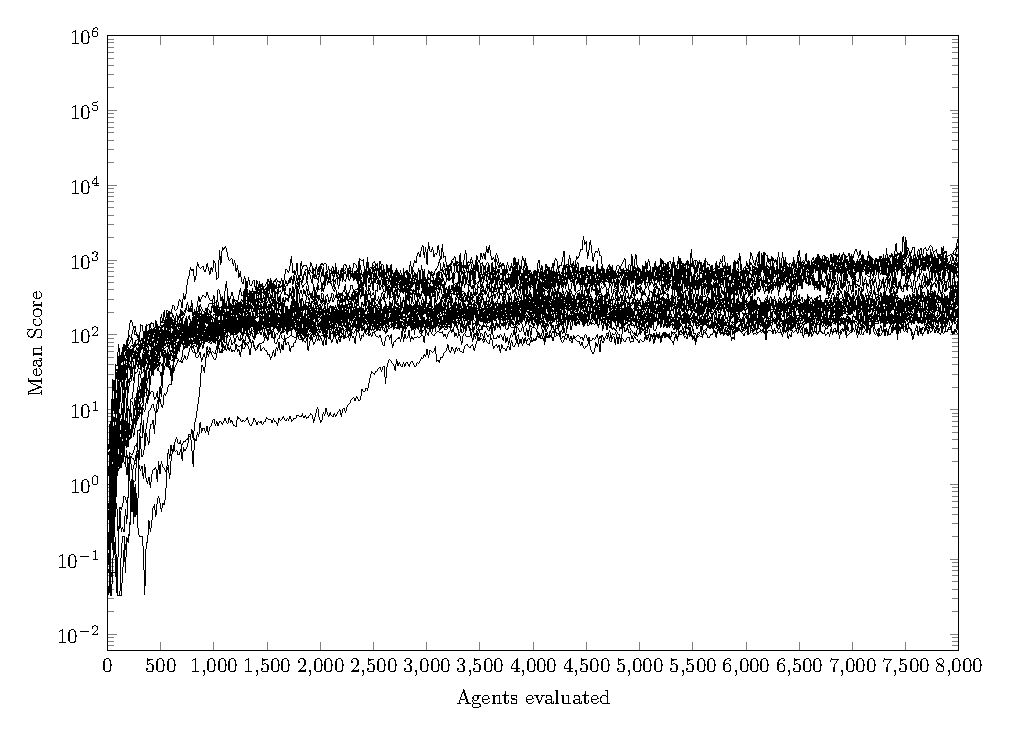
\includegraphics[width=\textwidth]{data/complexity/cma_hard/PlotFile.pdf}
    \end{subfigure} 
    \begin{subfigure}[b]{0.49\textwidth}
    	\caption{CMA-ES - Normal Tetris}
        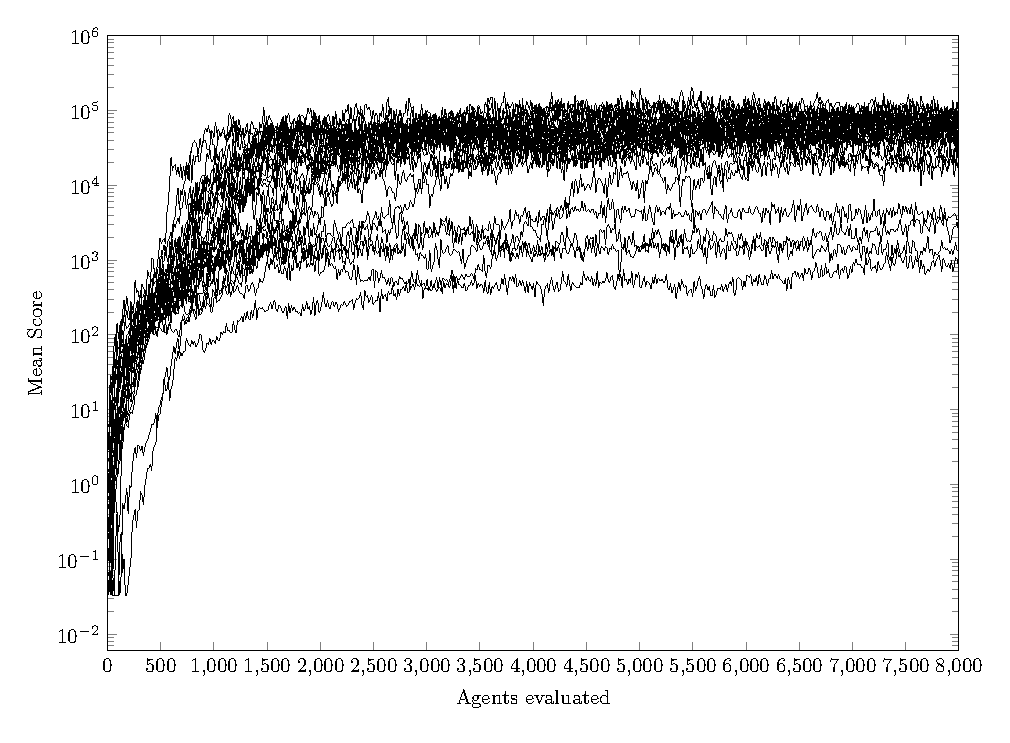
\includegraphics[width=\textwidth]{data/complexity/cma_normal/PlotFile.pdf}
    \end{subfigure}
    \begin{subfigure}[b]{0.49\textwidth}
    	\caption{Cross Entropy - Hard Tetris}
        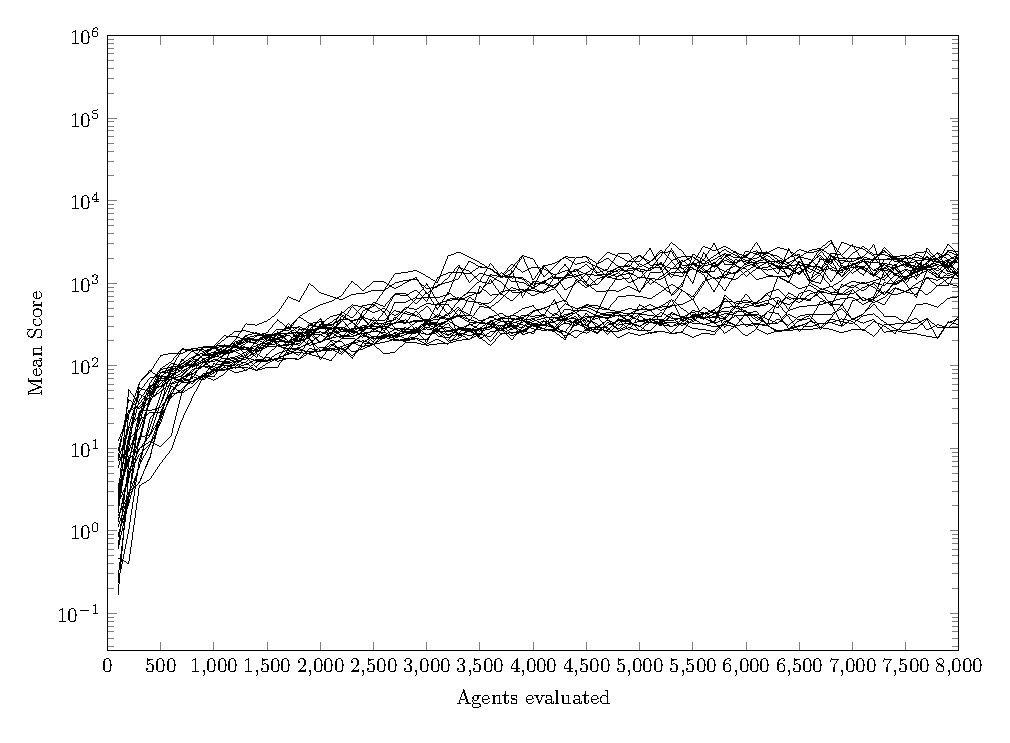
\includegraphics[width=\textwidth]{data/complexity/ce_hard/PlotFile.pdf}
    \end{subfigure}
    \begin{subfigure}[b]{0.49\textwidth}
    	\caption{Cross Entropy - Normal Tetris}
        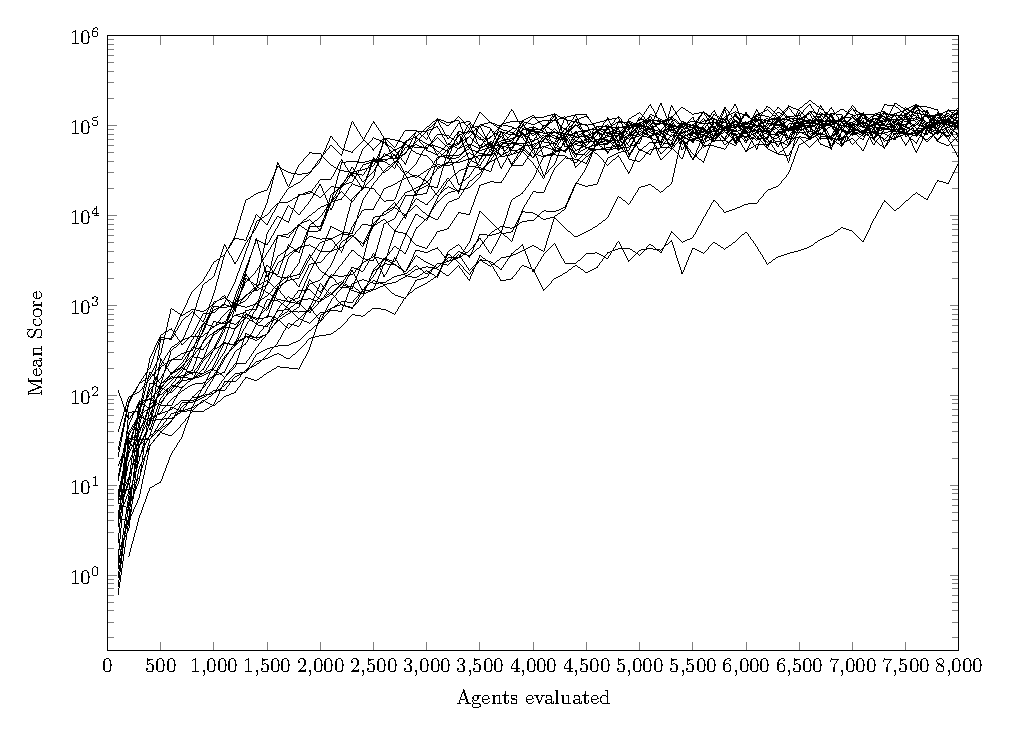
\includegraphics[width=\textwidth]{data/complexity/ce_normal/PlotFile.pdf}
    \end{subfigure}
    
    \caption{Complexity experiment results}
\end{figure}


\begin{table}[H]
\centering
\small
\begin{tabular}{c c c r r r r}
Tetris Type & Optimizer & mean & Q1 & Q2 & Q3\\
\hline
Hard & Cross Entropy & $1633.607$ & $1357.170$ & $1606.565$ & $1938.71$\\
Normal & Cross Entropy & $100059.463$ & $79357.440$ & $105999.500$ & $111047.500$\\
Hard & CMA-ES & $449.352$ & $201.850$ & $300.300$ & $529.350$\\
Normal & CMA-ES & $49760.161$ & $42528.740$ & $49915.700$ & $67764.729$\\
\end{tabular}
\caption{Quantile table of the complexity experiment results}
\end{table}

\begin{figure}[H]
\centering
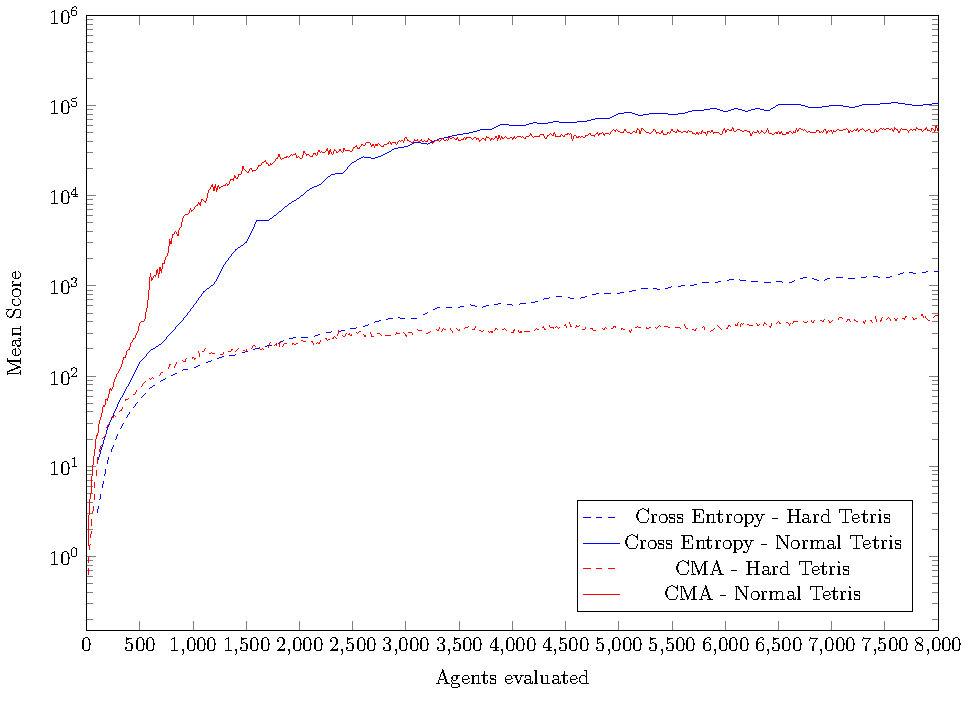
\includegraphics[scale=1]{data/complexity/mean/PlotFile.pdf}
\caption{Mean plots of the complexity experiment}
\end{figure}

\clearpage

\subsection{Comparison of feature sets}
Experiments to test the Bertsekas and Dellacherie feature sets in regards to achieved score. This will tell if a different feature set affects the algorithms performance. 

\begin{table}[h]
\centering
\small
\begin{tabular}{l r}
Optimizer & CMA-ES\\
Number of Evaluations & 8000\\
Number of Learning Games & 30\\
Population size& 13\\
Parent size & 6\\
Games per Agent & 1\\
Tetris Type & Hard\\
\hline
Recombination Type & Superlinear\\
Initial Sigma & $\frac{1}{\sqrt{22}}$\\
\quad & \quad
\end{tabular}
\quad
\begin{tabular}{l r}
Optimizer & Cross Entropy\\
Number of Evaluations & 8000\\
Number of Learning Games & 30\\
Population size & 100\\
Parent size & 10\\
Games per Agent & 1\\
Tetris Type & Hard\\
\hline
Sigma & 100\\
Noise Type & Constant\\
Noise & 4
\end{tabular}
\caption{Shark default CMA-ES and the Cross-entropy method}
\end{table}

%\comment{Add individual plots}

Used on the Bertsekas and Dellacherie feature sets

\begin{figure}[H]
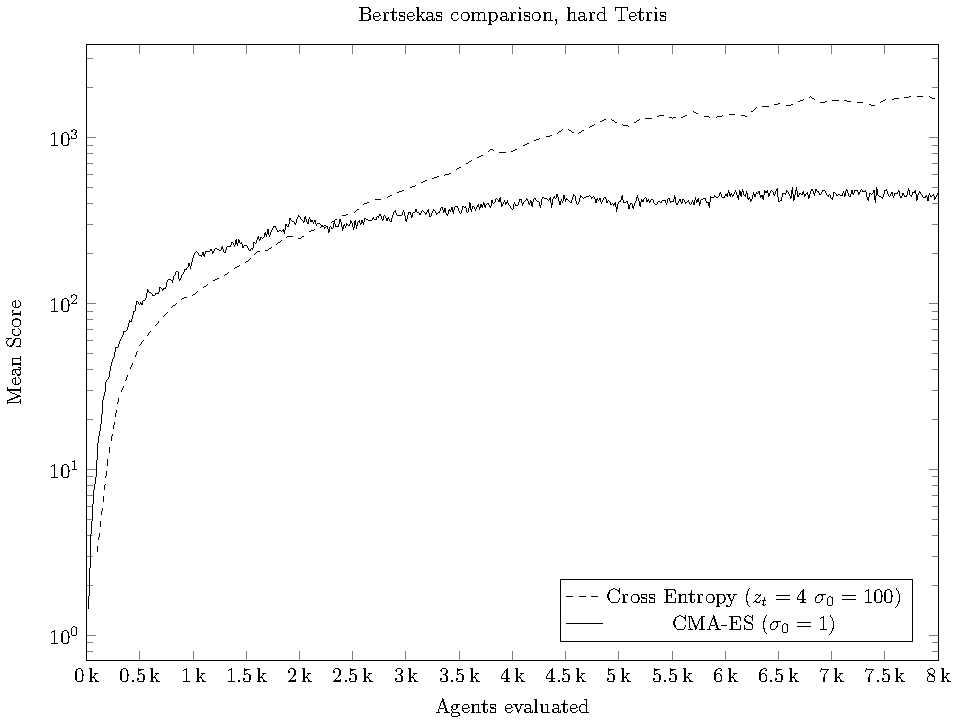
\includegraphics[scale=1]{plots/plotBertsekasCmaVsCEHardTetris}
\caption{Comparison between CMA-ES and the Cross-entropy method
using hard Tetris and the Bertsekas feature set}
%\label{fig:featuresetCompareBertsekas}}
\end{figure}

\begin{figure}[H]
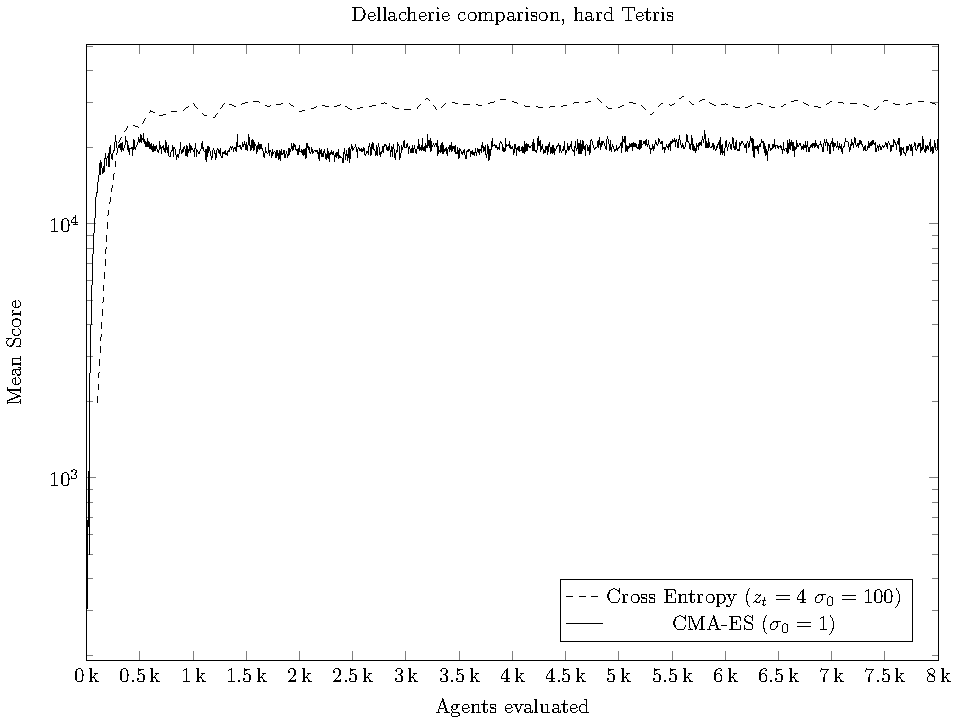
\includegraphics[scale=1]{plots/plotDellCmaVsCEHardTetris}
\caption{Comparison between CMA-ES and the Cross-entropy method
using hard Tetris and the Dellacherie feature set}
%\label{fig:Dellacherie}}
\end{figure}

\clearpage

\subsection{Verification of Cross Entropy}
Using the same configurations as in the experiments performed by Thiery and Scherrer \citep{scherrer2009}, we will reproduce the experiments to verify our implementation of the Cross-entropy method.\\
\\
\begin{table}[h!]
\centering
\begin{tabular}{l r}
Optimizer & Cross Entropy\\
Number of Evaluations & 8000\\
Population size & 100\\
Parent size & 10\\
Games per Agent & 1\\
Tetris Type & Normal\\
\hline
Sigma & 100\\
Noise Type & No noise\\
Noise & -
\end{tabular}
\caption{The Cross-entropy method - No noise}
\end{table}

\begin{table}[h!]
\centering
\begin{tabular}{l r}
Optimizer & Cross Entropy\\
Number of Evaluations & 8000\\
Population size & 100\\
Parent size & 10\\
Games per Agent & 1\\
Tetris Type & Normal\\
\hline
Sigma & 100\\
Noise Type & Constant\\
Noise & 4
\end{tabular}
\caption{The Cross-entropy method - Constant noise}
\end{table}

\begin{table}[h!]
\centering
\begin{tabular}{l r}
Optimizer & Cross Entropy\\
Number of Evaluations & 8000\\
Population size & 100\\
Parent size & 10\\
Games per Agent & 1\\
Tetris Type & Normal\\
\hline
Sigma & 100\\
Noise Type & Linear decreasing\\
Noise & $max \left( 5 - \frac{t}{10}, 0 \right)$
\end{tabular}
\caption{The Cross-entropy method - Linear decreasing noise}
\end{table}

\clearpage

\begin{figure}[H]
\begin{center}
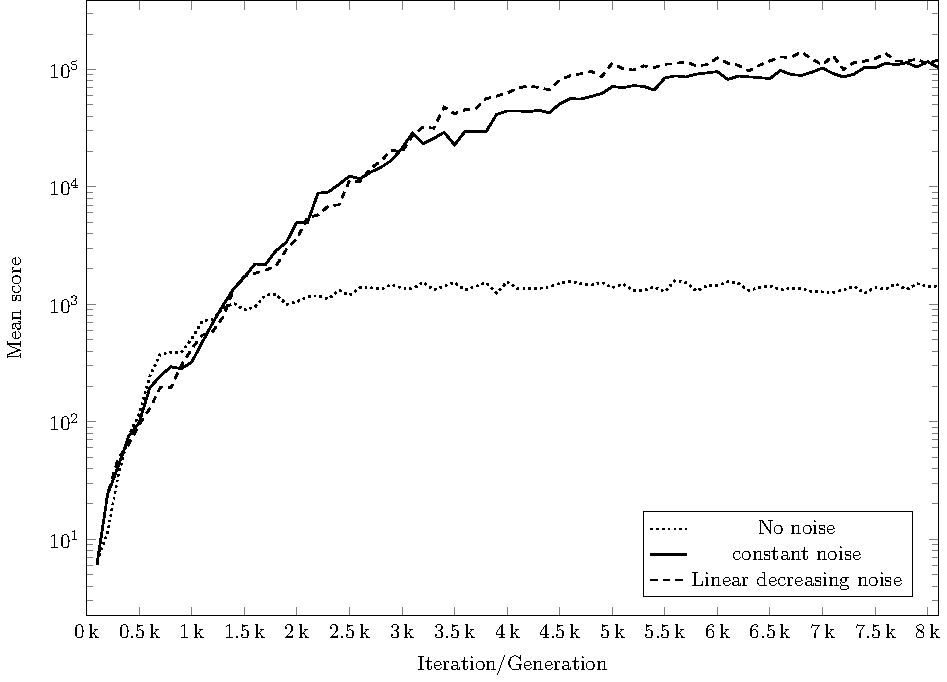
\includegraphics[scale=1]{plots/meansPlot}
\end{center}
\caption{The Cross-entropy method - mean performance of each configuration}
\end{figure}

\clearpage
\begin{figure}[H]
\begin{center}
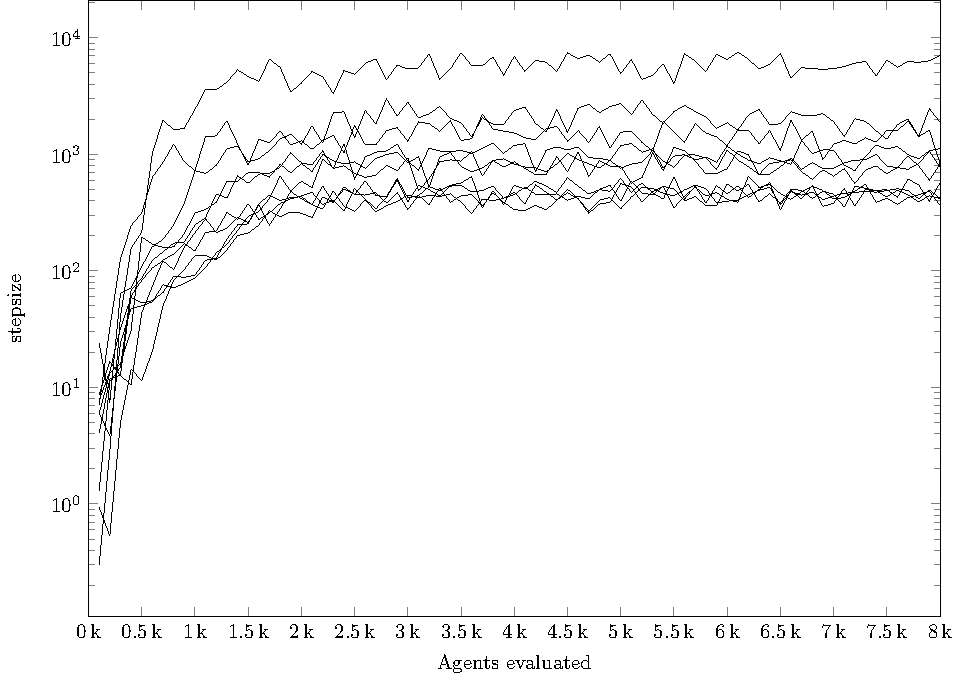
\includegraphics[scale=0.48]{plots/noNoisePlot}
\end{center}
\caption{The Cross-entropy method - No noise}
\end{figure}
\begin{figure}[H]
\begin{center}
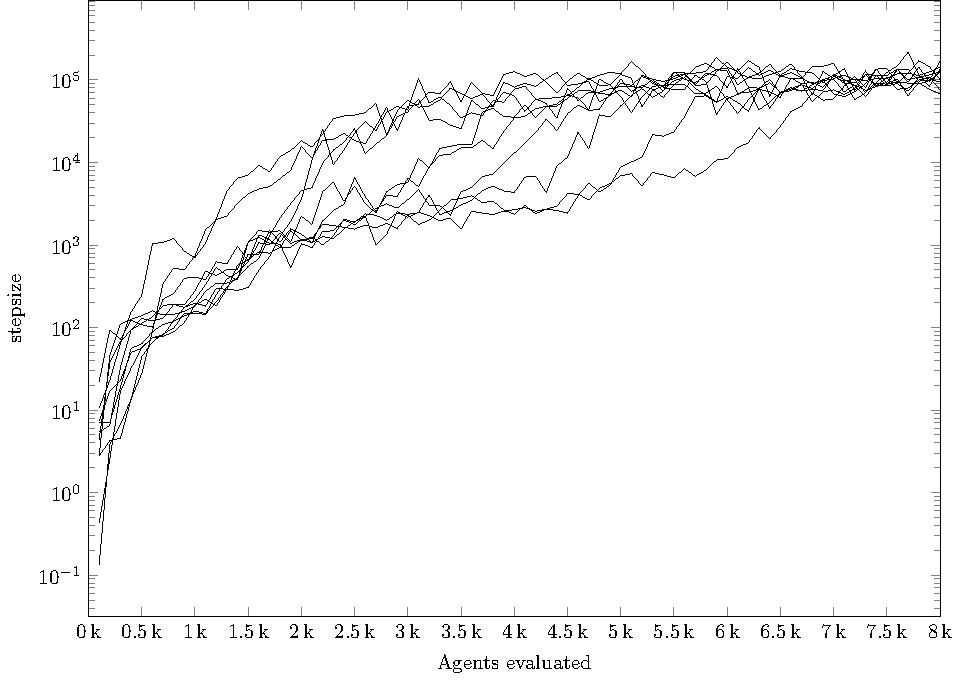
\includegraphics[scale=0.48]{plots/constantNoisePlot}
\end{center}
\caption{The Cross-entropy method - Constant noise}
\end{figure}
\begin{figure}[H]
\begin{center}
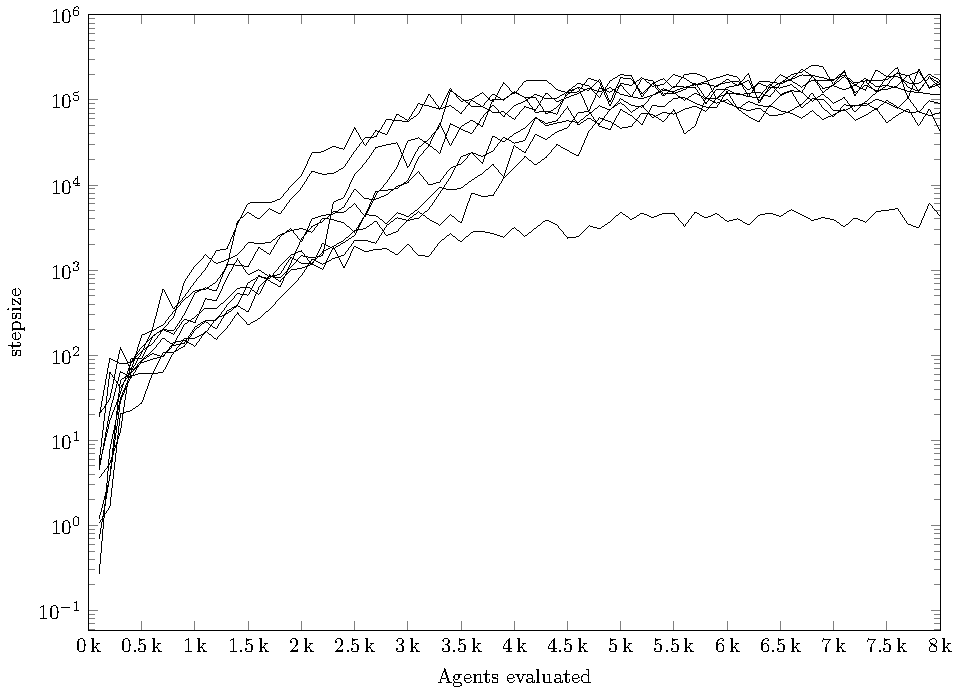
\includegraphics[scale=0.48]{plots/linearNoisePlot}
\end{center}
\caption{The Cross-entropy method - Linear decreasing noise}
\end{figure}


\clearpage

\subsection{The Cross-entropy method - Population and selection size \label{appendixCrossEntropyConfig}}
%\comment{Update plots and quantile table}\\
We want to investigate if there exists a better configuration than the 100/10 which was also previously used by other researchers.
The Cross-entropy method for the Tetris problem uses 10 \% Parent selection as standard. However, we will also test 25\% and 50\% Parent selection derived from configurations in CMA-ES. (This corresponds to the Parent selection for each of the three Recombination types)\\
\\
The general testing parameters are as follows
\begin{table}[h]
\centering
\begin{tabular}{l r}
Optimizer & Cross Entropy\\
Number of Evaluations & 8000\\
Population size & See table \ref{CEPopulationParentSize}\\
Parent size & See table \ref{CEPopulationParentSize}\\
Games per Agent & 1\\
Tetris Type & Normal\\
\hline
Sigma & 100\\
Noise Type & Constant\\
Noise & 4
\end{tabular}
\caption{General setup for Population/Parent size experiments for the Cross-entropy method}
\end{table}

with the following Population/Parent size

\begin{table}[h]
\centering
\begin{tabular}{r r}
Population size & Parent size\\
\hline
13 & 1\\
13 & 3\\
13 & 6\\
22 & 2\\
22 & 5\\
22 & 11\\
50 & 5\\
50 & 12\\
50 & 25\\
100 & 10\\
100 & 25\\
100 & 50\\
200 & 20\\
200 & 50\\
200 & 100
\end{tabular}
\caption{Population/Parent size \label{CEPopulationParentSize}}
\end{table}

\clearpage
Quantile table of of the results with 10 \%, 25 \% and 50 \% Parent size

\begin{figure}[H]
\centering
\begin{tabular}{r r | r r r r}
Population & Parent size & mean & Q1 & Q2 & Q3\\
\hline
13 & $10\%$  & 1585,3     & 93,0      & 113,5        & 220,7\\
13 & $25\%$  & 30.496,9   & 15.222,1  & 20.264,2     & 39.019,8\\
13 & $50\%$  & 39.824,2   & 26.457,0  & 33.663,4     & 49.743,7\\
22 & $10\%$  & 35.841,6   & 20.391,9  & 42.045,5     & 48.464,6\\
22 & $25\%$  & 80.884,9   & 56.042,5  & 71.900,2     & 78.653,4\\
22 & $50\%$  & 52.887,4   & 23.531,9  & 42.161,0     & 83.144,1\\
50 & $10\%$  & 95,623,1   & 82.738,9  & 93.388,9     & 111.351,5\\
50 & $25\%$  & 110.525,0  & 103.128,1 & 111.195,5    & 121.974,4\\
50 & $50\%$  & 69.130,7   & 52.511,0  & 64.351,6     & 91.488,6\\
100 & $10\%$ & 115.868,7  & 84.368,5  & 122.238,5    & 146.457,0\\
100 & $25\%$ & 70.011,1   & 58.008,0  & 69.588,2     & 80.432,7\\
100 & $50\%$ & 22.910,4   & 4.037,7   & 14.353,7     & 47.215,9\\
200 & $10\%$ & 85.181,7   & 45.201,5  & 96.803,1     & 117.578,0\\
200 & $25\%$ & 32.894,6   & 8688,7    & 25.333,1     & 58.434,8\\
200 & $50\%$ & 946,4      & 585,0     & 802,5        & 1.267,7
\end{tabular}
\caption{The Cross-entropy configuration test results - Quantile table}
\end{figure}


The plots from the configuration experiment of the Cross-entropy method.
All plots depicts the numbers of games played along the x-axis
and the mean score of the centroid agent along the y-axis.

\begin{tabular}{@{}l@{}l@{}}
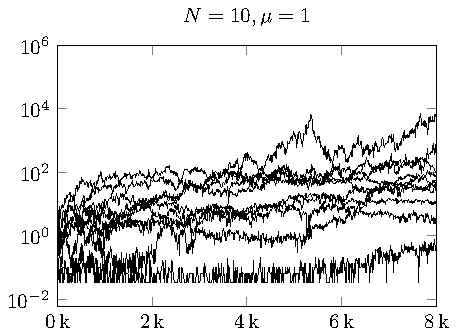
\includegraphics[scale=1]{plots/ce_ConstantNoise_l10_o1_all} &
\includegraphics[scale=1]{plots/ce_ConstantNoise_l13_o6_all} \\
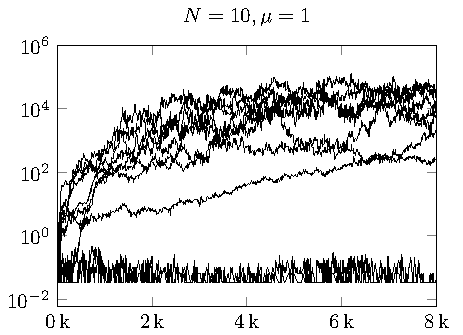
\includegraphics[scale=1]{plots/ce_ConstantNoise_l10_o5_all} &
\end{tabular}

\begin{tabular}{@{}l@{}l@{}}
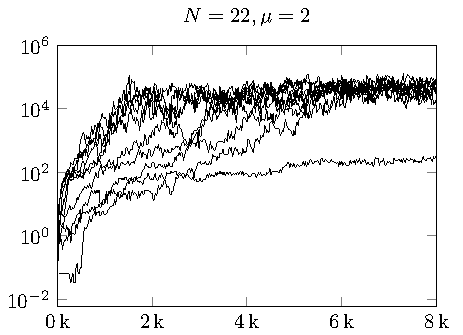
\includegraphics[scale=1]{plots/ce_ConstantNoise_l22_o2_all}&
\includegraphics[scale=1]{plots/ce_ConstantNoise_l22_o5_all}\\
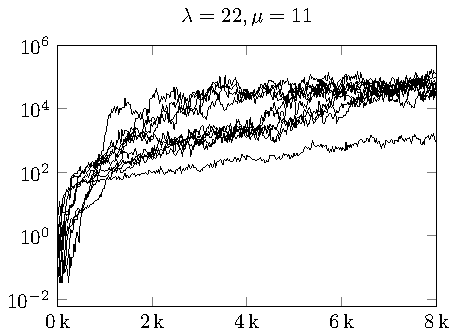
\includegraphics[scale=1]{plots/ce_ConstantNoise_l22_o11_all}
\end{tabular}

\begin{tabular}{@{}l@{}l@{}}
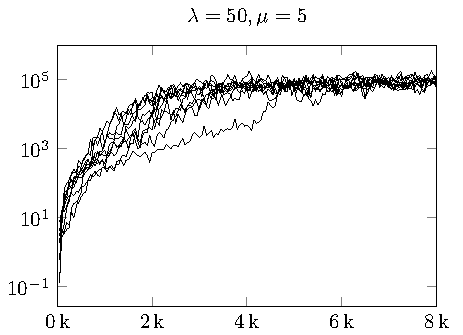
\includegraphics[scale=1]{plots/ce_ConstantNoise_l50_o5_all} &
\includegraphics[scale=1]{plots/ce_ConstantNoise_l50_o12_all} \\
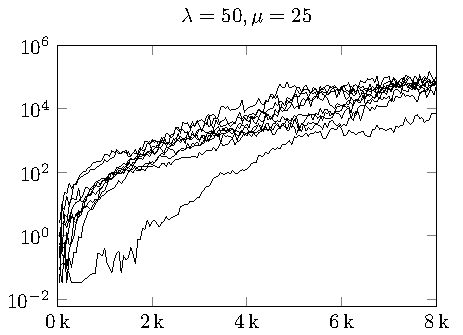
\includegraphics[scale=1]{plots/ce_ConstantNoise_l50_o25_all}
\end{tabular}

\begin{tabular}{@{}l@{}l@{}}
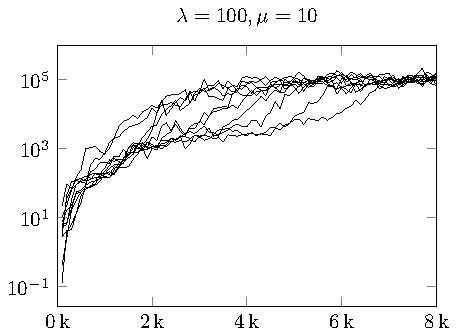
\includegraphics[scale=1]{plots/ce_ConstantNoise_l100_o10_all} &
\includegraphics[scale=1]{plots/ce_ConstantNoise_l100_o25_all} \\
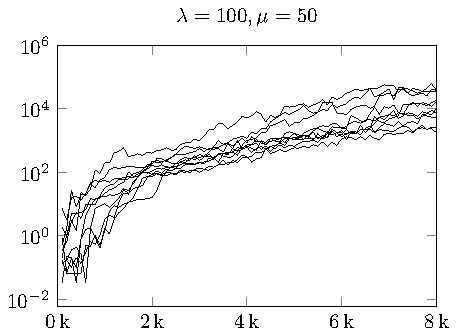
\includegraphics[scale=1]{plots/ce_ConstantNoise_l100_o50_all}
\end{tabular}

\begin{tabular}{@{}l@{}l@{}}
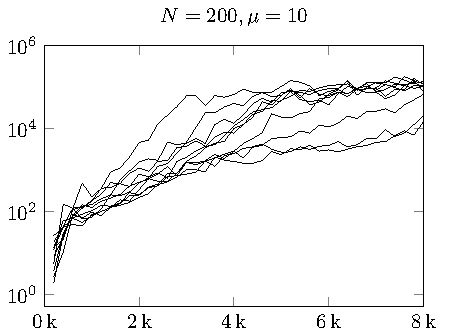
\includegraphics[scale=1]{plots/ce_ConstantNoise_l200_o20_all} &
\includegraphics[scale=1]{plots/ce_ConstantNoise_l200_o50_all} \\
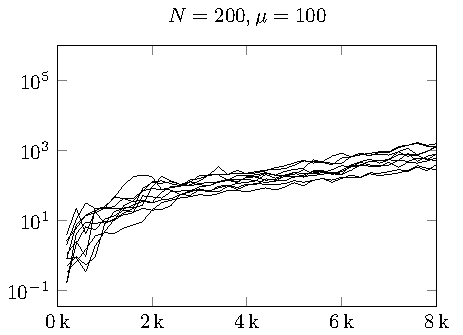
\includegraphics[scale=1]{plots/ce_ConstantNoise_l200_o100_all}
\end{tabular}


\clearpage

\subsection{Optimal settings for the Cross-entropy method - Games per agent \label{appendixCEPopulationParent}}
Experiments to determine the optimal number of games played per agent for best resulting
score at lowest evaluation cost. These experiments will utilize hard Tetris as game configuration, 
which was experimentally proven to be usable.

\begin{table}[h]
\centering
\begin{tabular}{l r}
Optimizer & Cross Entropy\\
Number of Evaluations & 80000\\
Population size & See table \ref{GamesPerAgentCE}\\
Parent size & See table \ref{GamesPerAgentCE}\\
Games per Agent & See table \ref{GamesPerAgentCE}\\
Tetris Type & Hard\\
\hline
Sigma & 100\\
Noise Type & Constant\\
Noise & 4
\end{tabular}
\caption{General setup for experiments with games per agent}
\end{table}

with the following Population/Parent size and number of games played per agent


\begin{table}[H]
\centering
\begin{tabular}{c c c}
Population Size & Parent size & Games per Agent\\
\hline
$13$ & $10\%$ & 1/3/5/7/10\\
$13$ & $25\%$ & 1/3/5/7/10\\
$13$ & $50\%$ & 1/3/5/7/10\\
$22$ & $10\%$ & 1/3/5/7/10\\
$22$ & $25\%$ & 1/3/5/7/10\\
$22$ & $50\%$ & 1/3/5/7/10\\
$50$ & $10\%$ & 1/3/5/7/10\\
$50$ & $25\%$ & 1/3/5/7/10\\
$50$ & $50\%$ & 1/3/5/7/10\\
$100$ & $10\%$ & 1/3/5/7/10\\
$100$ & $25\%$ & 1/3/5/7/10\\
$100$ & $50\%$ & 1/3/5/7/10\\
$200$ & $10\%$ & 1/3/5/7/10\\
$200$ & $25\%$ & 1/3/5/7/10\\
$200$ & $50\%$ & 1/3/5/7/10
\end{tabular}
\caption{Games per agent configurations for the Cross-entropy method experiments}
%\label{GamesPerAgentCE}}
\end{table}

\clearpage

\begin{figure}
	\centering
	\captionsetup[subfigure]{justification=centering}
    \begin{subfigure}[b]{0.49\textwidth}
    	\caption{Population size 13, Parent size 1}
        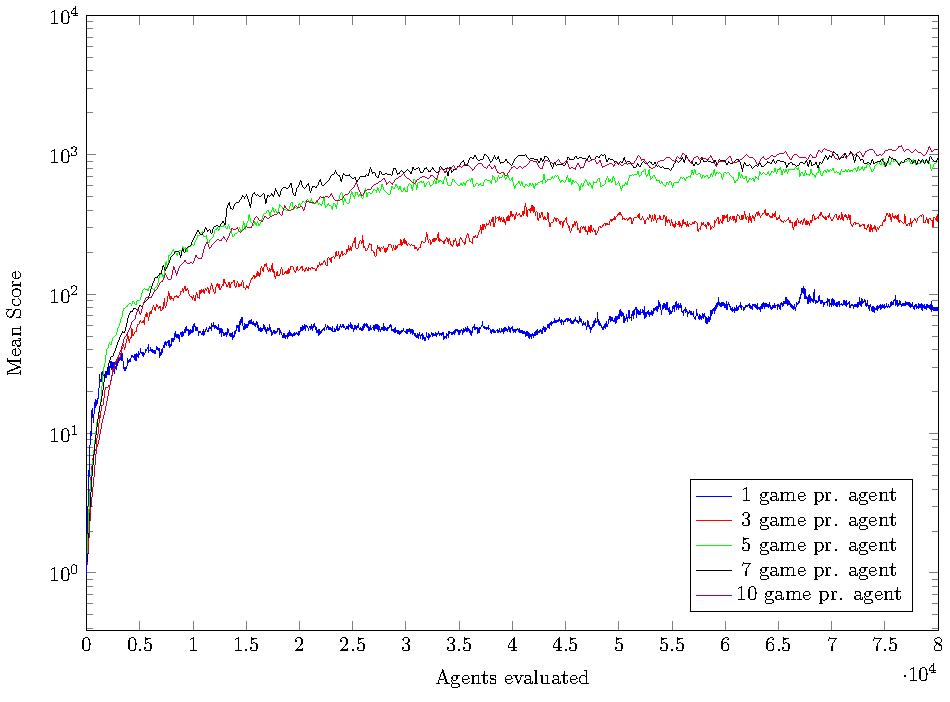
\includegraphics[width=\textwidth]{data/ce_population_offspring/13x_split/constant_l13_o1/mean/PlotFile.pdf}
    \end{subfigure} 
    \begin{subfigure}[b]{0.49\textwidth}
    	\caption{Population size 13, Parent size 3}
        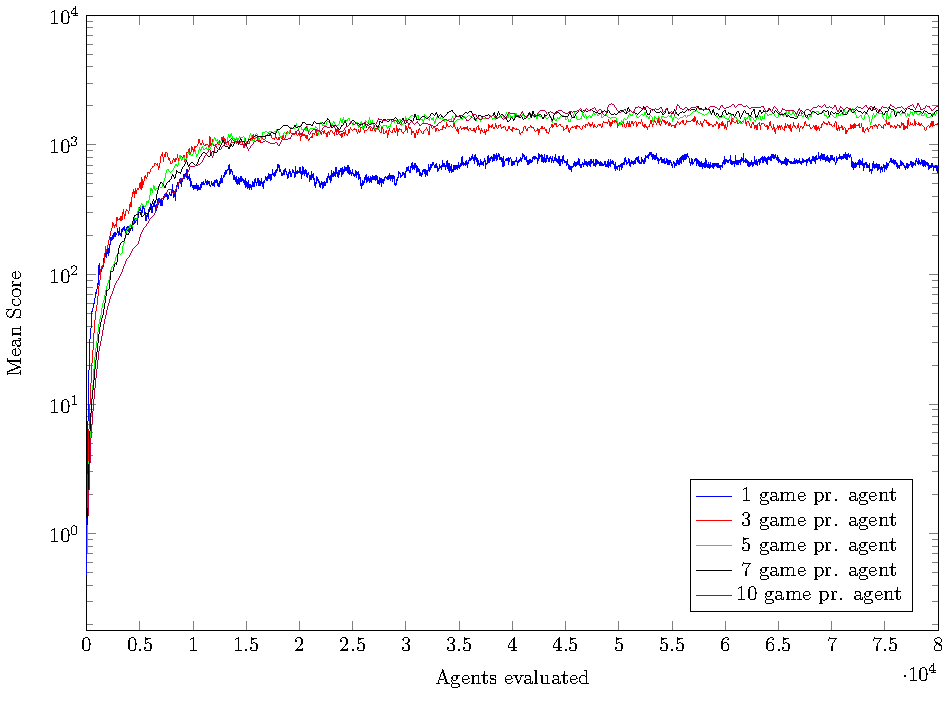
\includegraphics[width=\textwidth]{data/ce_population_offspring/13x_split/constant_l13_o3/mean/PlotFile.pdf}
    \end{subfigure}
    \begin{subfigure}[b]{0.49\textwidth}
    	\caption{Population size 13, Parent size 6}
        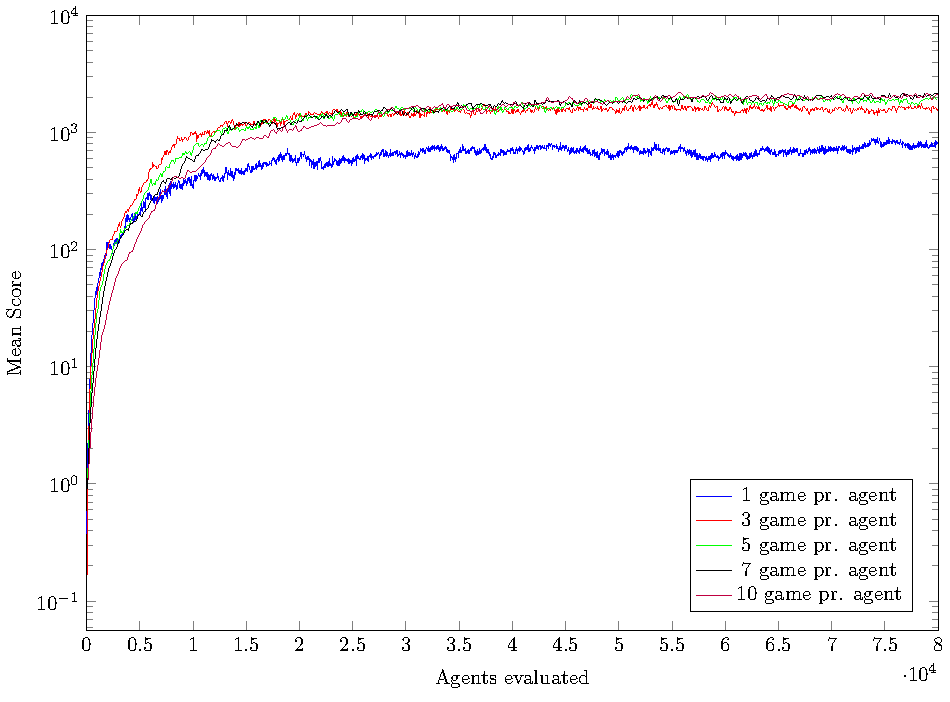
\includegraphics[width=\textwidth]{data/ce_population_offspring/13x_split/constant_l13_o6/mean/PlotFile.pdf}
    \end{subfigure}
    \begin{subfigure}[b]{0.49\textwidth}
    	\caption{Population size 22, Parent size 2}
        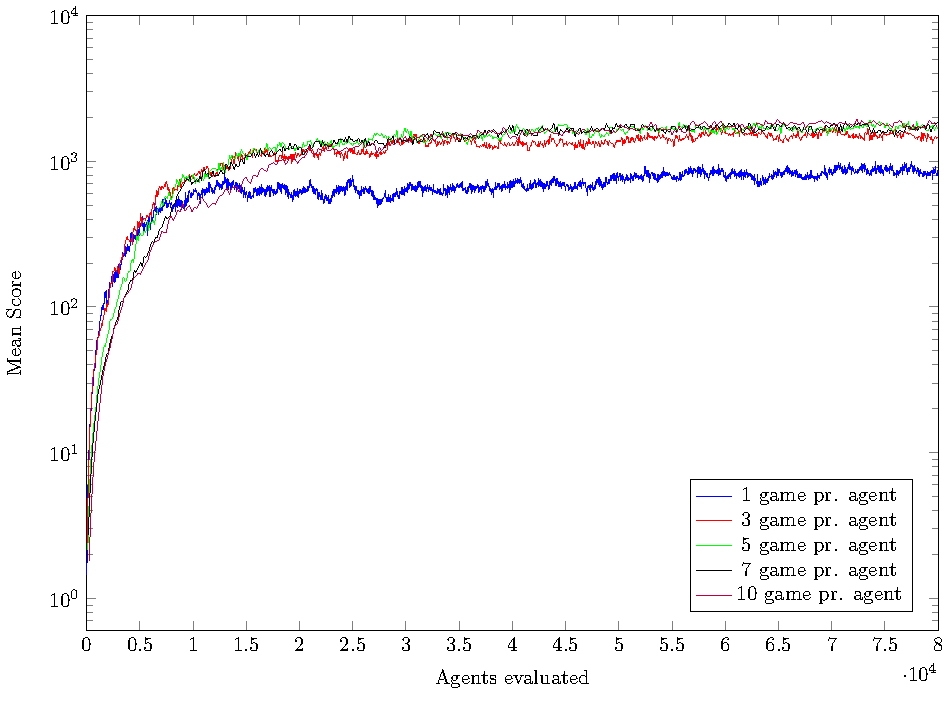
\includegraphics[width=\textwidth]{data/ce_population_offspring/22x_split/constant_l22_o2/mean/PlotFile.pdf}
    \end{subfigure}
    \begin{subfigure}[b]{0.49\textwidth}
    	\caption{Population size 22, Parent size 5}
        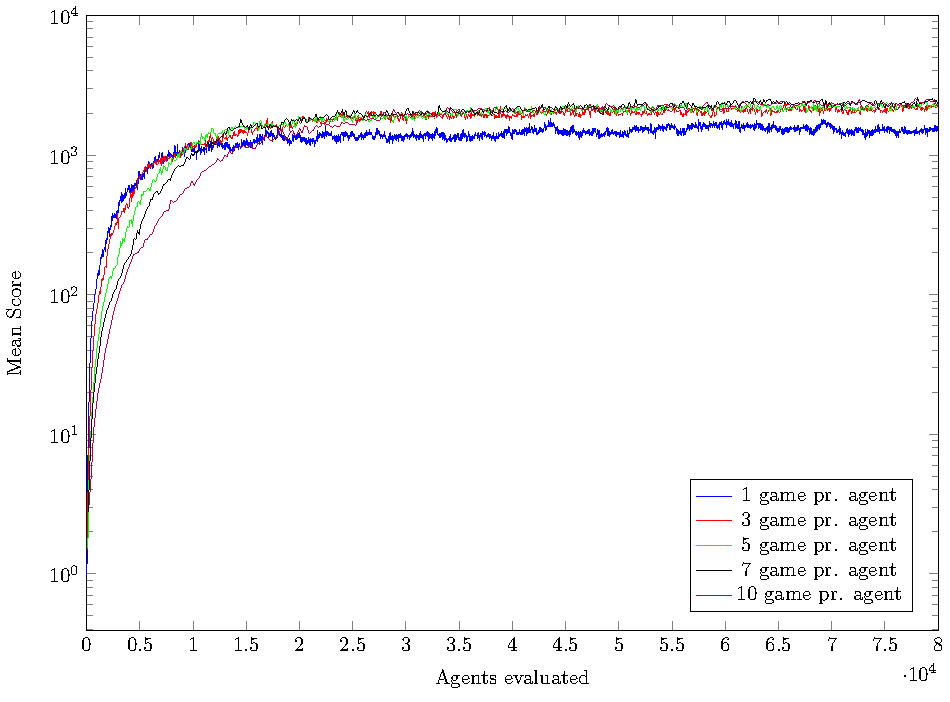
\includegraphics[width=\textwidth]{data/ce_population_offspring/22x_split/constant_l22_o5/mean/PlotFile.pdf}
    \end{subfigure}
    \begin{subfigure}[b]{0.49\textwidth}
    	\caption{Population size 22, Parent size 11}
        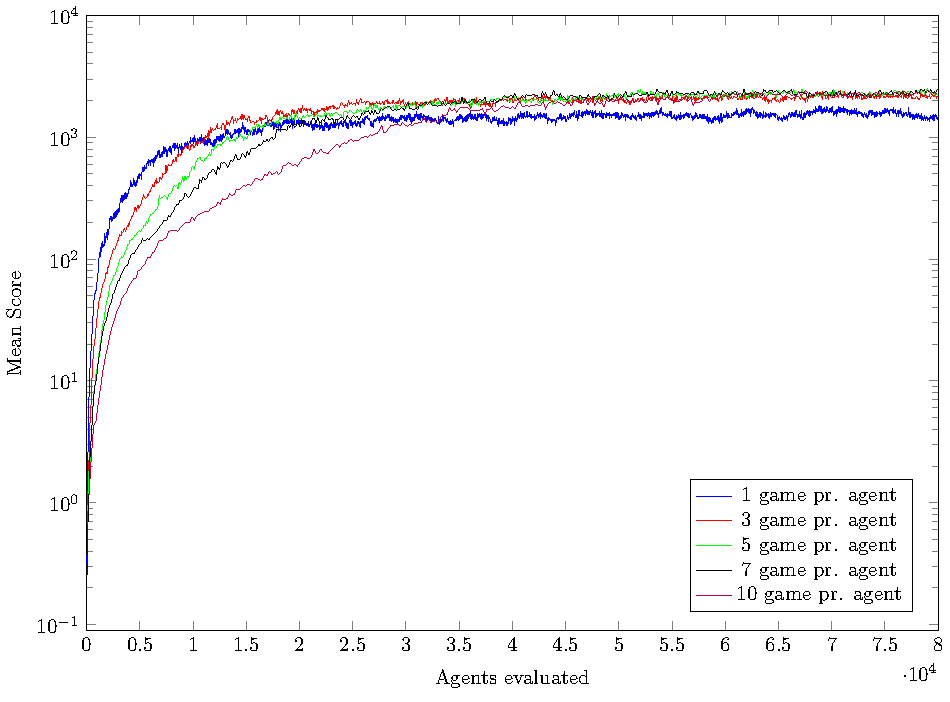
\includegraphics[width=\textwidth]{data/ce_population_offspring/22x_split/constant_l22_o11/mean/PlotFile.pdf}
    \end{subfigure}
    
    \caption{Mean results for Population size 13 and 22 with parent sizes $10 \% , 25 \%$ and $50 \%$}
\end{figure}

\clearpage

\begin{figure}
	\centering
	\captionsetup[subfigure]{justification=centering}
    \begin{subfigure}[b]{0.49\textwidth}
    	\caption{Population size 50, Parent size 5}
        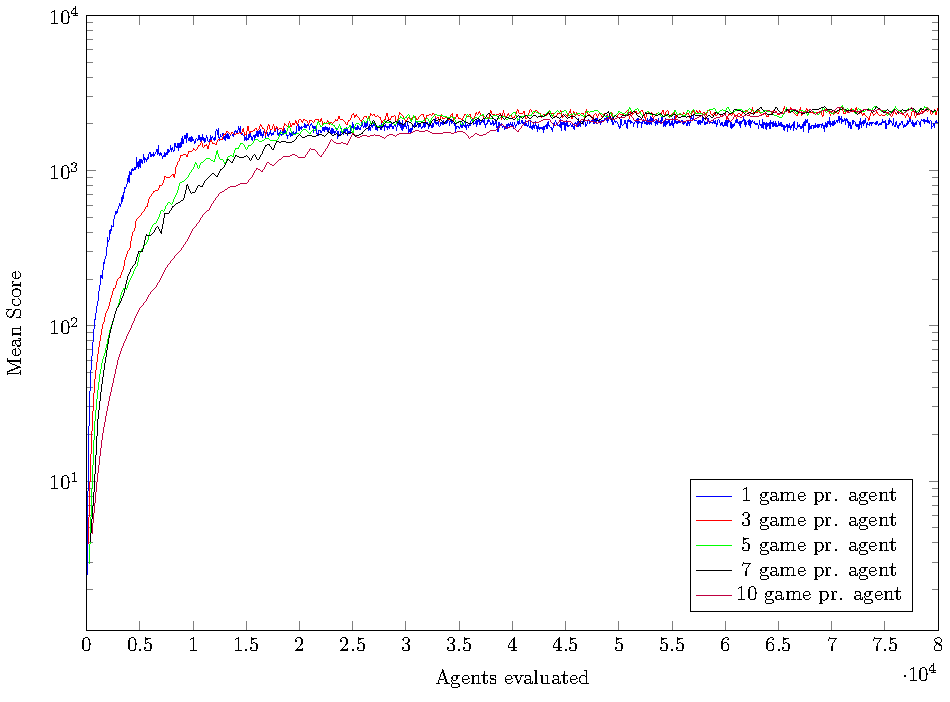
\includegraphics[width=\textwidth]{data/ce_population_offspring/50x_split/constant_l50_o5/mean/PlotFile.pdf}
    \end{subfigure} 
    \begin{subfigure}[b]{0.49\textwidth}
    	\caption{Population size 50, Parent size 12}
        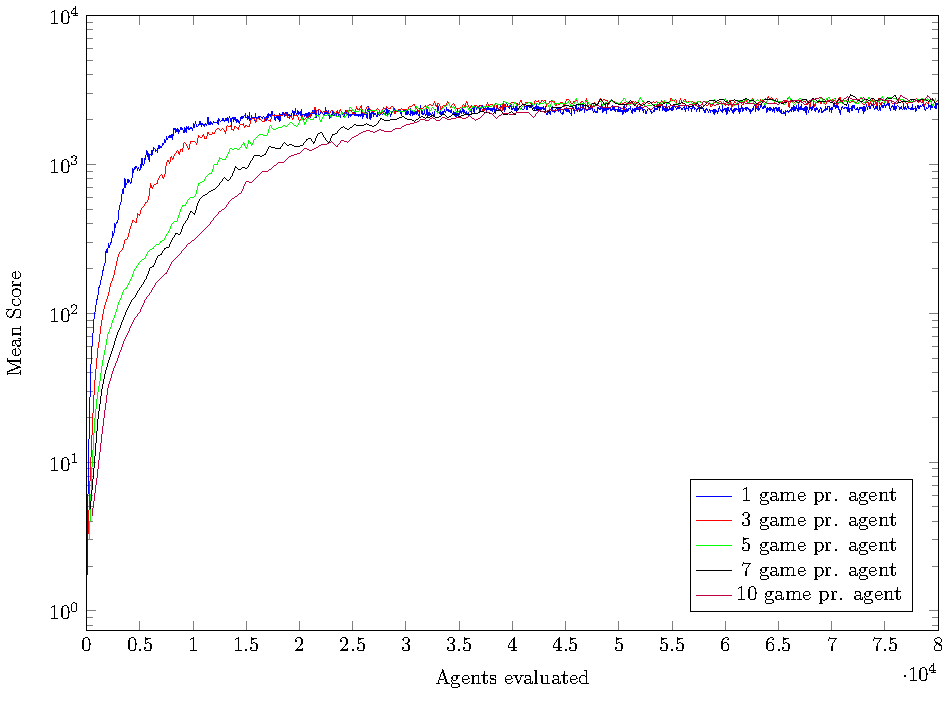
\includegraphics[width=\textwidth]{data/ce_population_offspring/50x_split/constant_l50_o12/mean/PlotFile.pdf}
    \end{subfigure}
    \begin{subfigure}[b]{0.49\textwidth}
    	\caption{Population size 50, Parent size 25}
        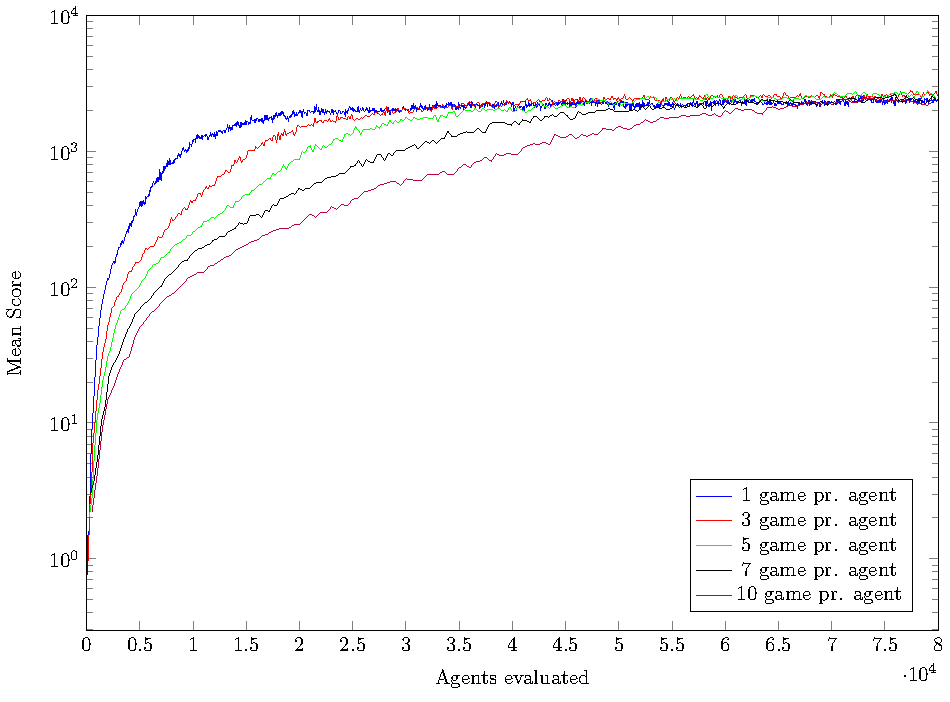
\includegraphics[width=\textwidth]{data/ce_population_offspring/50x_split/constant_l50_o25/mean/PlotFile.pdf}
    \end{subfigure}
    \begin{subfigure}[b]{0.49\textwidth}
    	\caption{Population size 100, Parent size 10}
        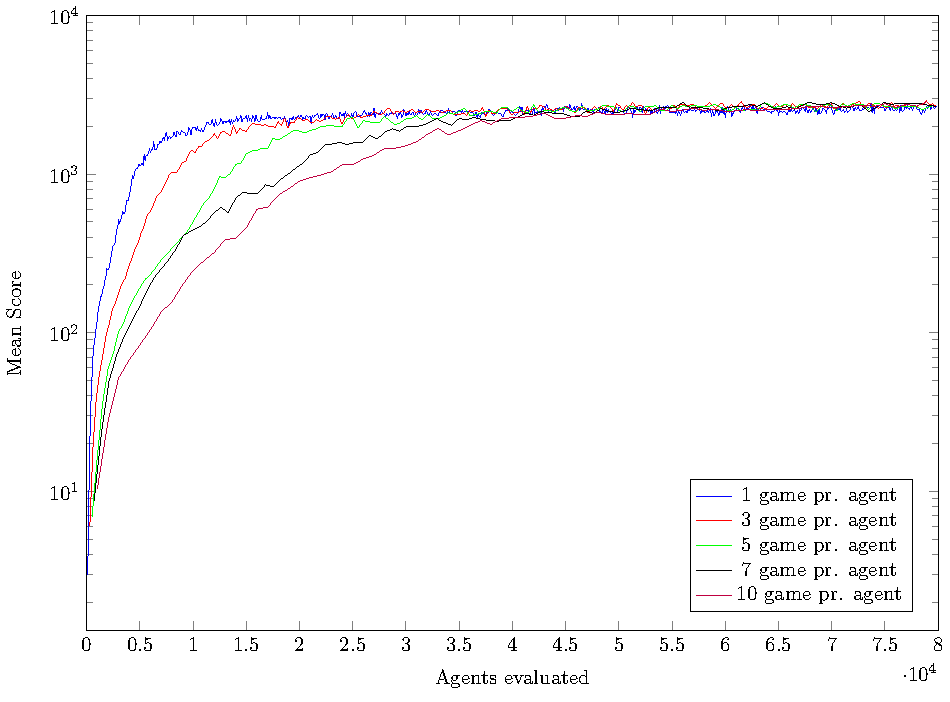
\includegraphics[width=\textwidth]{data/ce_population_offspring/100x_split/constant_l100_o10/mean/PlotFile.pdf}
    \end{subfigure}
    \begin{subfigure}[b]{0.49\textwidth}
    	\caption{Population size 100, Parent size 25}
        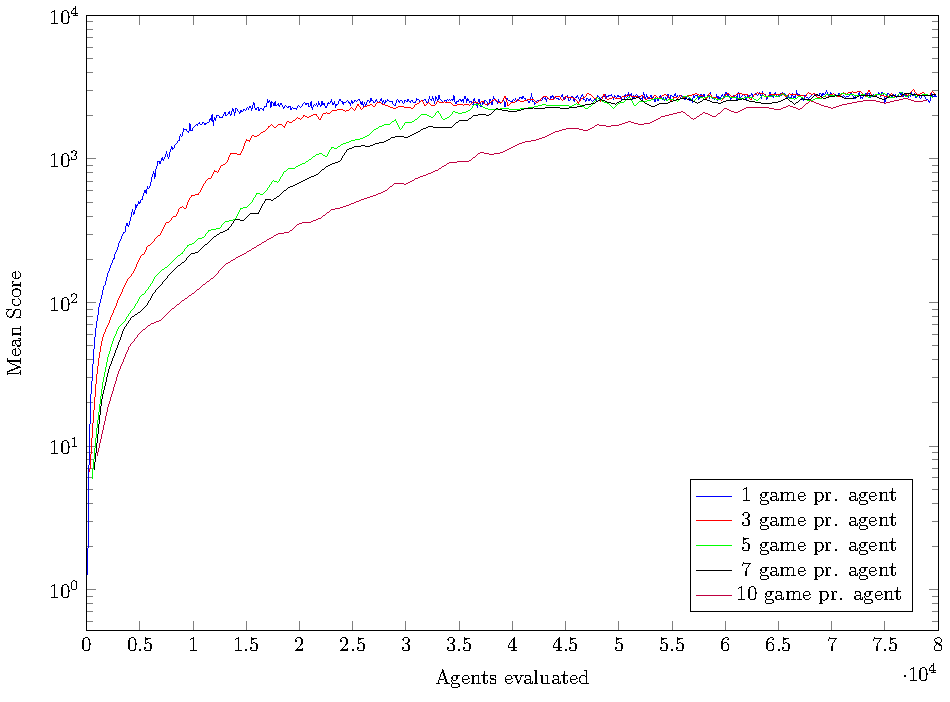
\includegraphics[width=\textwidth]{data/ce_population_offspring/100x_split/constant_l100_o25/mean/PlotFile.pdf}
    \end{subfigure}
    \begin{subfigure}[b]{0.49\textwidth}
    	\caption{Population size 100, Parent size 50}
        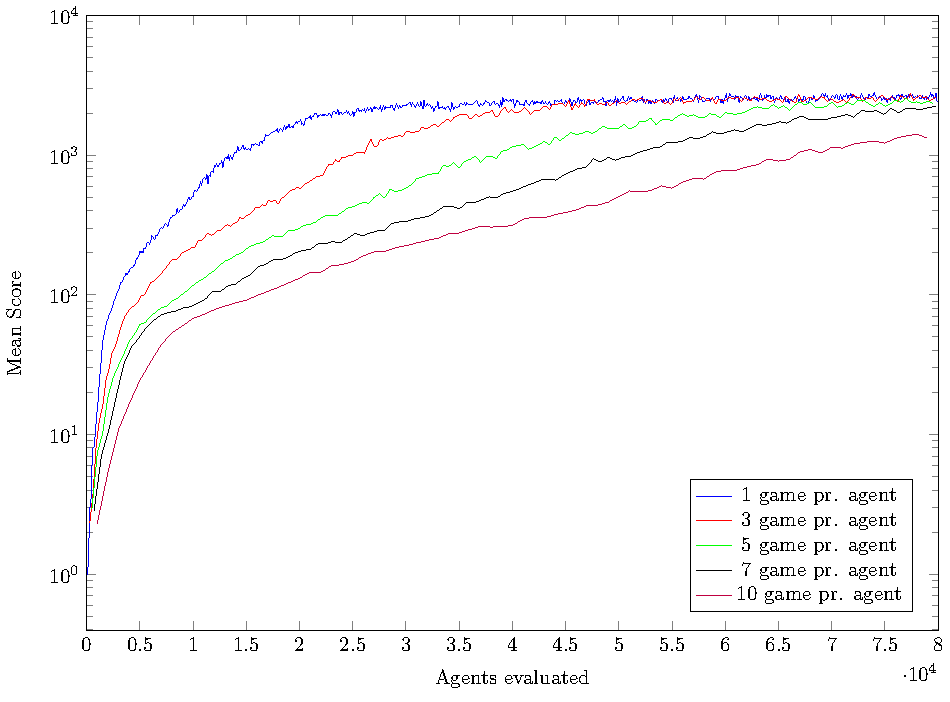
\includegraphics[width=\textwidth]{data/ce_population_offspring/100x_split/constant_l100_o50/mean/PlotFile.pdf}
    \end{subfigure}
    
    \caption{Mean results for Population size 50 and 100 with parent sizes $10 \% , 25 \%$ and $50 \%$}
\end{figure}

\clearpage

\begin{figure}
	\captionsetup[subfigure]{justification=centering}
    \begin{subfigure}[b]{0.49\textwidth}
    	\caption{Population size 200, Parent size 20}
        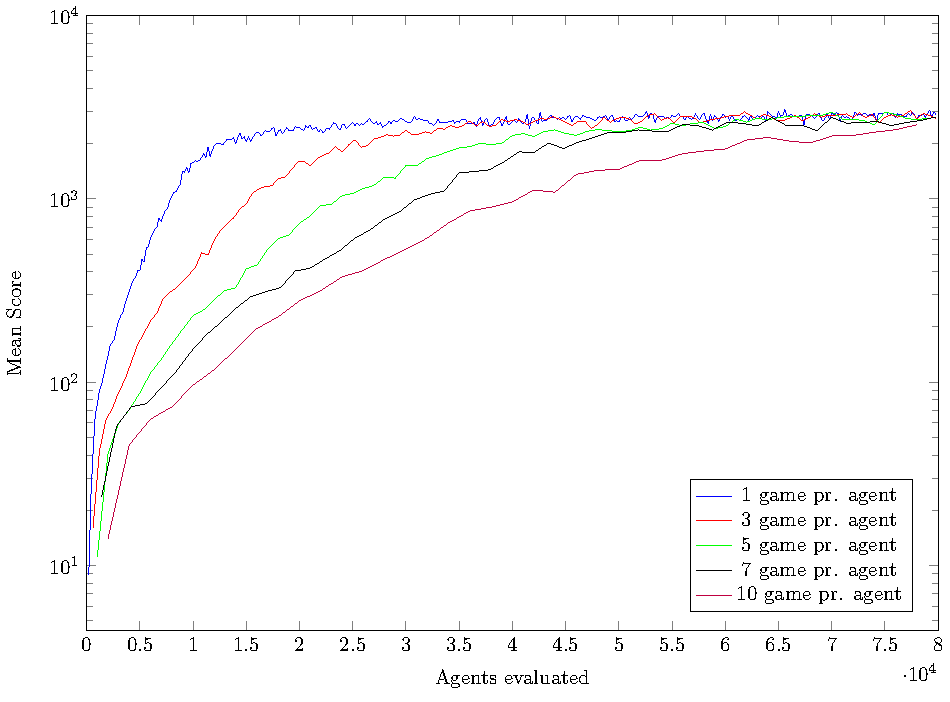
\includegraphics[width=\textwidth]{data/ce_population_offspring/200x_split/constant_l200_o20/mean/PlotFile.pdf}
    \end{subfigure} 
    \begin{subfigure}[b]{0.49\textwidth}
    	\caption{Population size 200, Parent size 50}
        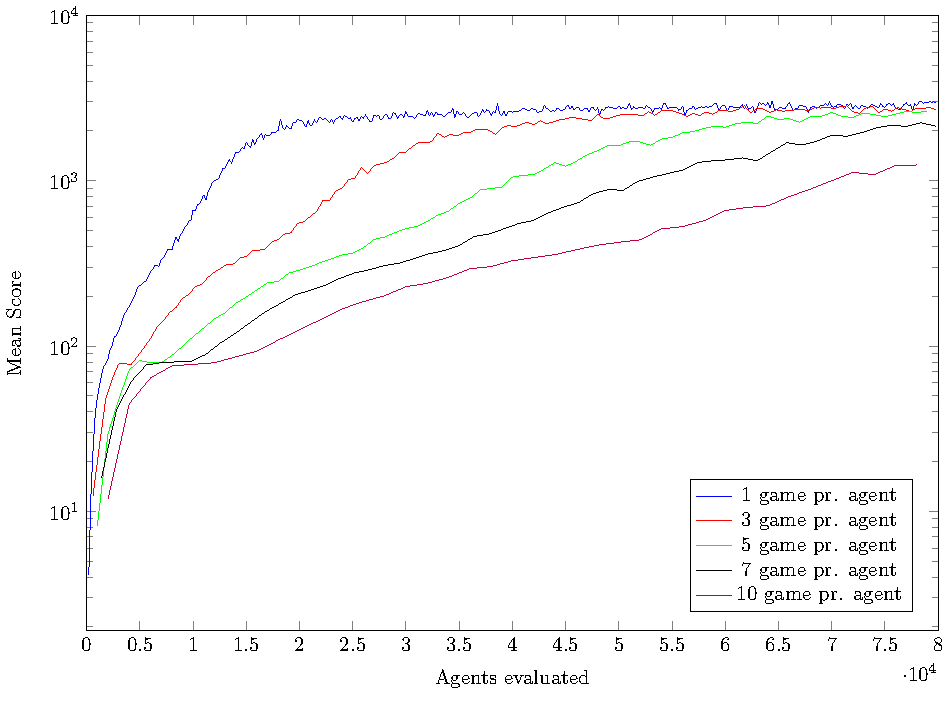
\includegraphics[width=\textwidth]{data/ce_population_offspring/200x_split/constant_l200_o50/mean/PlotFile.pdf}
    \end{subfigure}
    \begin{subfigure}[b]{0.49\textwidth}
    	\caption{Population size 200, Parent size 100}
        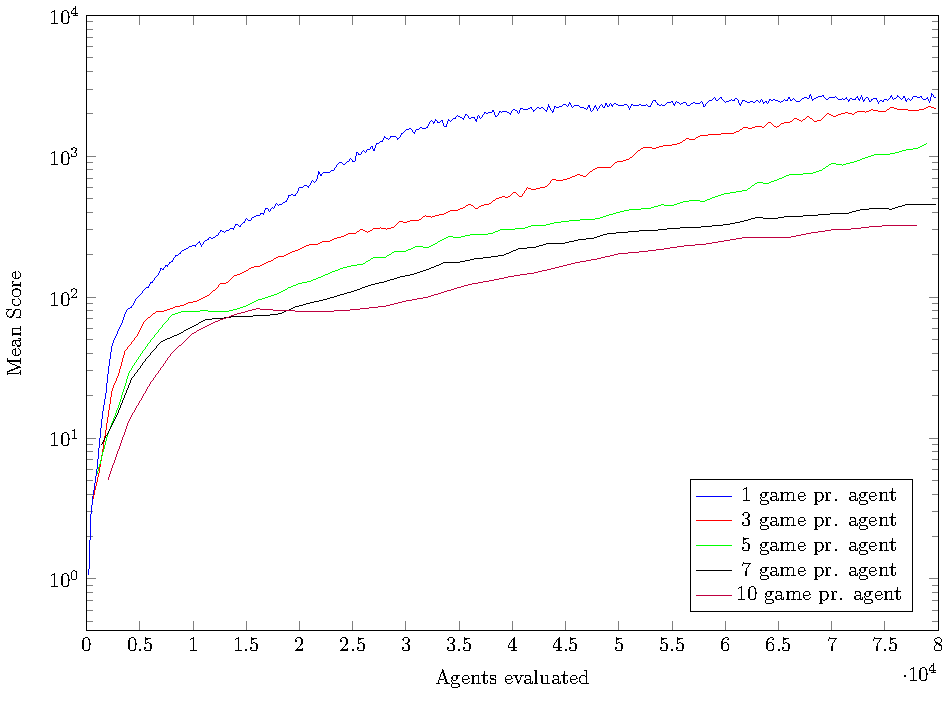
\includegraphics[width=\textwidth]{data/ce_population_offspring/200x_split/constant_l200_o100/mean/PlotFile.pdf}
    \end{subfigure}
    
    \caption{Mean results for Population size 200 with parent sizes $10 \% , 25 \%$ and $50 \%$}
\end{figure}

\clearpage

\begin{table}[H]
\centering
\small
\begin{tabular}{c c c r r r r}
Population & Parent & Games per Agent & mean & Q1 & Q2 & Q3\\
\hline
$13$ & $1$ & 1 & $76.402$ & $46.143$ & $58.850$ & $87.786$\\
$13$ & $1$ & 3 & $329.847$ & $180.787$ & $266.633$ & $418.630$\\
$13$ & $1$ & 5 & $870.593$ & $648.593$ & $870.466$ & $1047.998$\\
$13$ & $1$ & 7 & $951.487$ & $646.383$ & $915.418$ & $1130.101$\\
\hdashline
$13$ & $1$ & 10 & $1098.654$ & $834.683$ & $939.150$ & $1270.262$\\
\hdashline
$13$ & $3$ & 1 & $681.930$ & $451.493$ & $615.583$ & $777.900$\\
$13$ & $3$ & 3 & $1485.366$ & $1260.690$ & $1497.965$ & $1582.008$\\
$13$ & $3$ & 5 & $1779.540$ & $1448.080$ & $1764.150$ & $2103.521$\\
$13$ & $3$ & 7 & $1844.008$ & $1635.631$ & $1790.465$ & $2025.209$\\
\hdashline
$13$ & $3$ & 10 & $1992.749$ & $1566.989$ & $1965.365$ & $2381.089$\\
\hdashline
$13$ & $6$ & 1 & $814.019$ & $598.073$ & $736.783$ & $966.0269$\\
$13$ & $6$ & 3 & $1595.290$ & $1219.319$ & $1504.700$ & $1870.699$\\
$13$ & $6$ & 5 & $1981.514$ & $1695.181$ & $1927.700$ & $2151.810$\\
\hdashline
$13$ & $6$ & 7 & $2173.595$ & $1818.110$ & $2105.500$ & $2398.201$\\
\hdashline
$13$ & $6$ & 10 & $2129.880$ & $1825.599$ & $2058.970$ & $2391.860$\\
\hdashline
\end{tabular}
\caption{Population 12 - The Cross-entropy method}
\end{table}

\begin{table}[H]
\centering
\small
\begin{tabular}{c c c r r r r}
Population & Parent & Games per Agent & mean & Q1 & Q2 & Q3\\
\hline
$22$ & $2$ & 1 & $849.001$ & $542.797$ & $799.083$ & $1031.299$\\
$22$ & $2$ & 3 & $1442.883$ & $1276.870$ & $1437.550$ & $1541.938$\\
$22$ & $2$ & 5 & $1668.974$ & $1352.250$ & $1579.885$ & $1849.210$\\
\hdashline
$22$ & $2$ & 7 & $1843.644$ & $1575.732$ & $1860.815$ & $2112.678$\\
\hdashline
$22$ & $2$ & 10 & $1732.664$ & $1475.000$ & $1754.785$ & $2024.980$\\
$22$ & $5$ & 1 & $1485.692$ & $1202.661$ & $1561.635$ & $1661.268$\\
$22$ & $5$ & 3 & $2250.239$ & $2081.798$ & $2210.850$ & $2435.021$\\
\hdashline
$22$ & $5$ & 5 & $2371.793$ & $2013.168$ & $2412.815$ & $2708.931$\\
\hdashline
$22$ & $5$ & 7 & $2351.371$ & $1976.141$ & $2274.180$ & $2586.641$\\
$22$ & $5$ & 10 & $2266.329$ & $2010.798$ & $2175.850$ & $2365.220$\\
$22$ & $11$ & 1 & $1415.511$ & $1011.101$ & $1327.030$ & $1600.599$\\
$22$ & $11$ & 3 & $2168.012$ & $1966.552$ & $2119.100$ & $2456.230$\\
$22$ & $11$ & 5 & $2245.854$ & $2017.992$ & $2222.900$ & $2424.450$\\
\hdashline
$22$ & $11$ & 7 & $2463.227$ & $2091.090$ & $2384.230$ & $2702.740$\\
\hdashline
$22$ & $11$ & 10 & $2282.032$ & $1957.148$ & $2257.285$ & $2565.950$\\
\end{tabular}
\caption{Population 22 - The Cross-entropy method}
\end{table}


\begin{table}[H]
\centering
\small
\begin{tabular}{c c c r r r r}
Population & Parent & Games per Agent & mean & Q1 & Q2 & Q3\\
\hline
$50$ & $5$ & 1 & $2060.069$ & $1731.441$ & $1967.465$ & $2076.389$\\
\hdashline
$50$ & $5$ & 3 & $2524.279$ & $2195.189$ & $2501.985$ & $2848.859$\\
\hdashline
$50$ & $5$ & 5 & $2418.023$ & $2283.708$ & $2388.770$ & $2639.078$\\
$50$ & $5$ & 7 & $2433.615$ & $2145.718$ & $2356.800$ & $2734.611$\\
$50$ & $5$ & 10 & $2341.267$ & $2104.480$ & $2252.570$ & $2418.809$\\
$50$ & $12$ & 1 & $2563.539$ & $2283.399$ & $2502.880$ & $2830.192$\\
$50$ & $12$ & 3 & $2702.266$ & $2322.849$ & $2565.365$ & $2841.160$\\
\hdashline
$50$ & $12$ & 5 & $2749.991$ & $2605.171$ & $2702.400$ & $2835.960$\\
\hdashline
$50$ & $12$ & 7 & $2527.792$ & $2287.091$ & $2476.965$ & $2758.970$\\
$50$ & $12$ & 10 & $2687.438$ & $2342.811$ & $2577.285$ & $2838.771$\\
$50$ & $25$ & 1 & $2396.866$ & $2115.161$ & $2357.980$ & $2664.099$\\
\hdashline
$50$ & $25$ & 3 & $2572.860$ & $2308.748$ & $2615.185$ & $2861.858$\\
\hdashline
$50$ & $25$ & 5 & $2485.564$ & $2226.889$ & $2419.080$ & $2747.609$\\
$50$ & $25$ & 7 & $2396.309$ & $2180.099$ & $2306.165$ & $2605.832$\\
$50$ & $25$ & 10 & $2332.305$ & $2019.738$ & $2268.415$ & $2561.252$\\
\end{tabular}
\caption{Population 50 - The Cross-entropy method}
\end{table}



\begin{table}[H]
\centering
\small
\begin{tabular}{c c c r r r r}
Population & Parent & Games per Agent & mean & Q1 & Q2 & Q3\\
\hline
$100$ & $10$ & 1 & $2658.689$ & $2469.169$ & $2601.480$ & $2866.970$\\
$100$ & $10$ & 3 & $2677.629$ & $2375.419$ & $2770.615$ & $3004.819$\\
$100$ & $10$ & 5 & $2690.802$ & $2360.800$ & $2646.920$ & $2946.831$\\
$100$ & $10$ & 7 & $2678.393$ & $2442.688$ & $2630.120$ & $2877.830$\\
\hdashline
$100$ & $10$ & 10 & $2880.385$ & $2636.640$ & $2828.880$ & $3108.429$\\
\hdashline
$100$ & $25$ & 1 & $2702.678$ & $2443.269$ & $2692.620$ & $2973.202$\\
\hdashline
$100$ & $25$ & 3 & $2776.560$ & $2397.691$ & $2742.950$ & $3027.541$\\
\hdashline
$100$ & $25$ & 5 & $2666.479$ & $2469.161$ & $2673.770$ & $2917.939$\\
$100$ & $25$ & 7 & $2555.354$ & $2187.871$ & $2461.220$ & $2866.030$\\
$100$ & $25$ & 10 & $2823.755$ & $2540.171$ & $2729.280$ & $2933.510$\\
$100$ & $50$ & 1 & $2409.168$ & $2206.828$ & $2299.435$ & $2534.019$\\
\hdashline
$100$ & $50$ & 3 & $2622.402$ & $2318.410$ & $2714.500$ & $2905.521$\\
\hdashline
$100$ & $50$ & 5 & $2351.742$ & $2213.480$ & $2410.500$ & $2532.500$\\
$100$ & $50$ & 7 & $2232.970$ & $2035.291$ & $2296.430$ & $2466.811$\\
$100$ & $50$ & 10 & $1320.906$ & $1088.809$ & $1231.050$ & $1618.431$\\
\end{tabular}
\caption{Population 100 - The Cross-entropy method}
\end{table}


\begin{table}[H]
\centering
\small
\begin{tabular}{c c c r r r r}
Population & Parent & Games per Agent & mean & Q1 & Q2 & Q3\\
\hline
\hdashline
$200$ & $20$ & 1 & $2880.572$ & $2596.999$ & $2764.400$ & $3184.290$\\
\hdashline
$200$ & $20$ & 3 & $2735.539$ & $2493.400$ & $2751.215$ & $2849.329$\\
$200$ & $20$ & 5 & $2756.202$ & $2609.579$ & $2728.885$ & $2826.881$\\
$200$ & $20$ & 7 & $2797.015$ & $2515.971$ & $2722.150$ & $3036.839$\\
$200$ & $20$ & 10 & $2531.674$ & $2186.629$ & $2652.365$ & $2897.672$\\
\hdashline
$200$ & $50$ & 1 & $2950.767$ & $2564.118$ & $2841.065$ & $3377.189$\\
\hdashline
$200$ & $50$ & 3 & $2677.694$ & $2414.600$ & $2559.765$ & $2803.289$\\
$200$ & $50$ & 5 & $2627.598$ & $2296.710$ & $2641.415$ & $2999.199$\\
$200$ & $50$ & 7 & $2140.359$ & $1884.261$ & $2173.235$ & $2418.772$\\
$200$ & $50$ & 10 & $1245.519$ & $625.930$ & $1009.132$ & $1644.630$\\
\hdashline
$200$ & $100$ & 1 & $2589.020$ & $2391.080$ & $2594.285$ & $2798.470$\\
\hdashline
$200$ & $100$ & 3 & $2164.732$ & $2018.790$ & $2136.900$ & $2335.079$\\
$200$ & $100$ & 5 & $1235.709$ & $837.947$ & $1195.730$ & $1478.081$\\
$200$ & $100$ & 7 & $451.171$ & $377.813$ & $421.150$ & $498.470$\\
$200$ & $100$ & 10 & $320.356$ & $287.023$ & $322.733$ & $350.773$\\
\end{tabular}
\caption{Population 200 - The Cross-entropy method}
\end{table}

\clearpage

\begin{table}[H]
\centering
\small
\begin{tabular}{c c c r r r r}
Population & Parent & Games per Agent & mean & Q1 & Q2 & Q3\\
\hline
$13$ & $1$ & 10 & $1098.654$ & $834.683$ & $939.150$ & $1270.262$\\
$13$ & $3$ & 10 & $1992.749$ & $1566.989$ & $1965.365$ & $2381.089$\\
$13$ & $6$ & 7 & $2173.595$ & $1818.110$ & $2105.500$ & $2398.201$\\
\end{tabular}
\caption{Population 13 - The Cross-entropy method}
\end{table}

\begin{figure}[H]
\centering
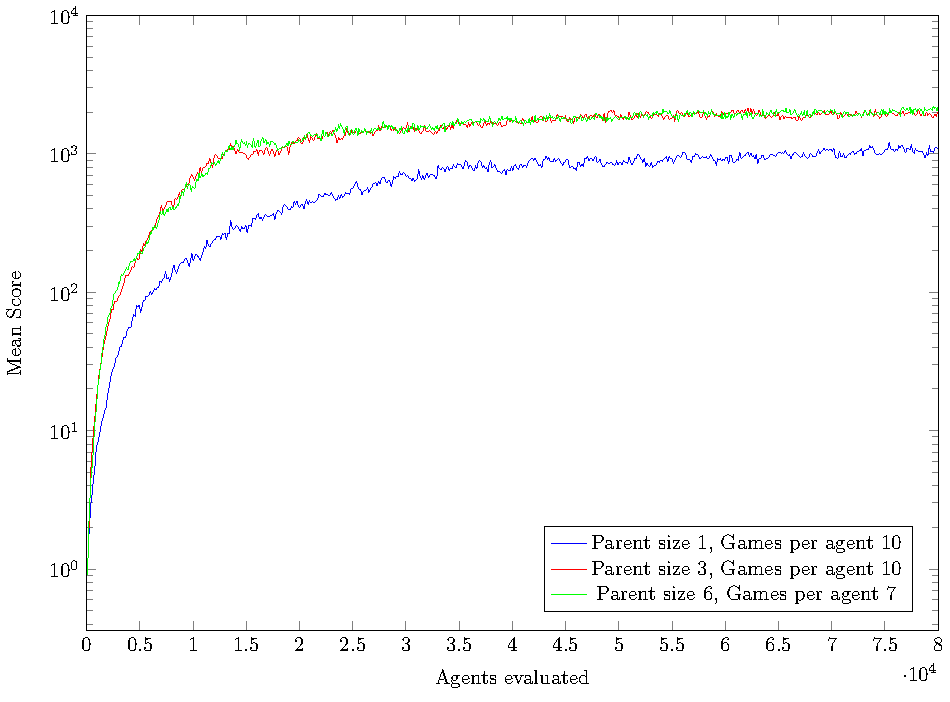
\includegraphics[scale=1]{data/ce_population_offspring/bestofeach_population/13x/PlotFile.pdf}
\caption{Best performing configurations for Population size 13}
\end{figure}

\clearpage

\begin{table}[H]
\centering
\small
\begin{tabular}{c c c r r r r}
Population & Parent & Games per Agent & mean & Q1 & Q2 & Q3\\
\hline
$22$ & $2$ & 7 & $1843.644$ & $1575.732$ & $1860.815$ & $2112.678$\\
$22$ & $5$ & 5 & $2371.793$ & $2013.168$ & $2412.815$ & $2708.931$\\
$22$ & $11$ & 7 & $2463.227$ & $2091.090$ & $2384.230$ & $2702.740$\\
\end{tabular}
\caption{Population 22 - The Cross-entropy method}
\end{table}

\begin{figure}[H]
\centering
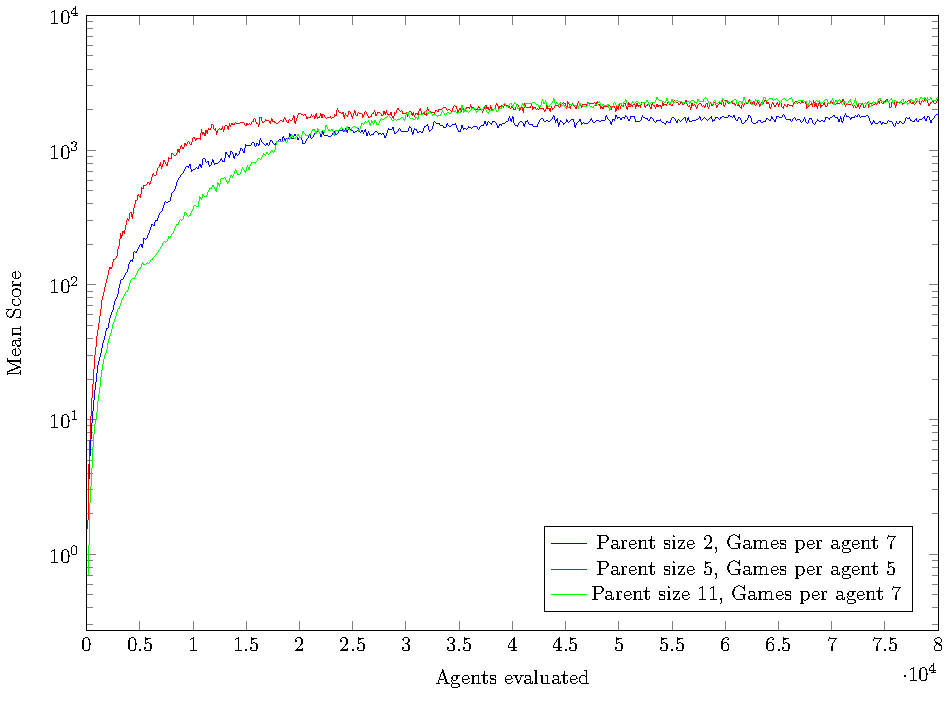
\includegraphics[scale=1]{data/ce_population_offspring/bestofeach_population/22x/PlotFile.pdf}
\caption{Best performing configurations for Population size 22}
\end{figure}

\clearpage

\begin{table}[H]
\centering
\small
\begin{tabular}{c c c r r r r}
Population & Parent & Games per Agent & mean & Q1 & Q2 & Q3\\
\hline
$50$ & $5$ & 3 & $2524.279$ & $2195.189$ & $2501.985$ & $2848.859$\\
$50$ & $12$ & 5 & $2749.991$ & $2605.171$ & $2702.400$ & $2835.960$\\
$50$ & $25$ & 3 & $2572.860$ & $2308.748$ & $2615.185$ & $2861.858$\\
\end{tabular}
\caption{Population 50 - The Cross-entropy method}
\end{table}

\begin{figure}[H]
\centering
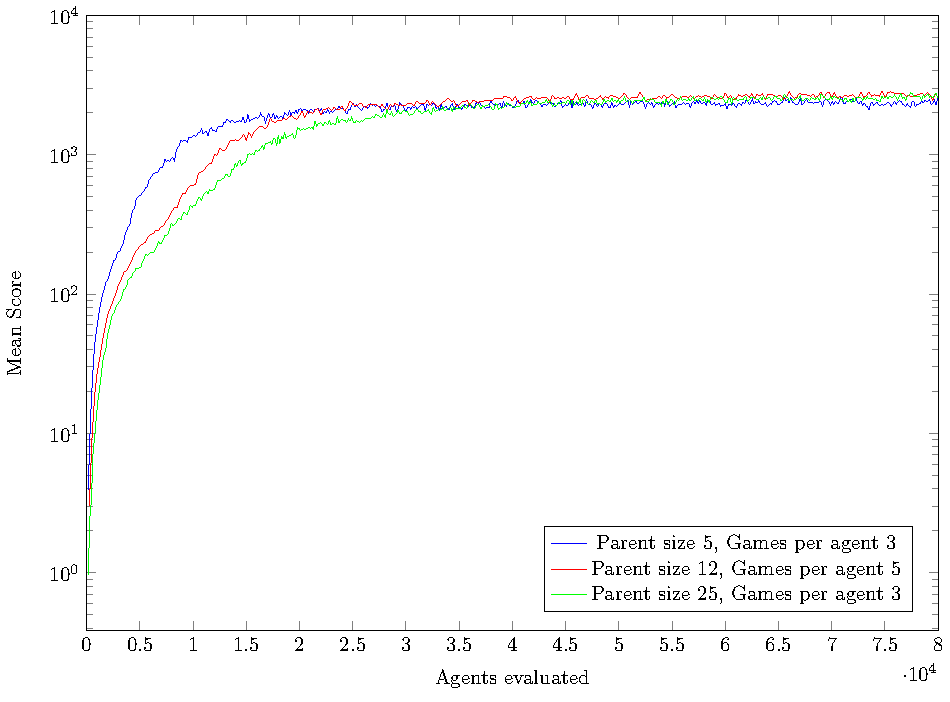
\includegraphics[scale=1]{data/ce_population_offspring/bestofeach_population/50x/PlotFile.pdf}
\caption{Best performing configurations for Population size 50}
\end{figure}

\clearpage

\begin{table}[H]
\centering
\small
\begin{tabular}{c c c r r r r}
Population & Parent & Games per Agent & mean & Q1 & Q2 & Q3\\
\hline
$100$ & $10$ & 10 & $2880.385$ & $2636.640$ & $2828.880$ & $3108.429$\\
$100$ & $25$ & 3 & $2776.560$ & $2397.691$ & $2742.950$ & $3027.541$\\
$100$ & $50$ & 3 & $2622.402$ & $2318.410$ & $2714.500$ & $2905.521$\\
\end{tabular}
\caption{Population 100 - The Cross-entropy method}
\end{table}

\begin{figure}[H]
\centering
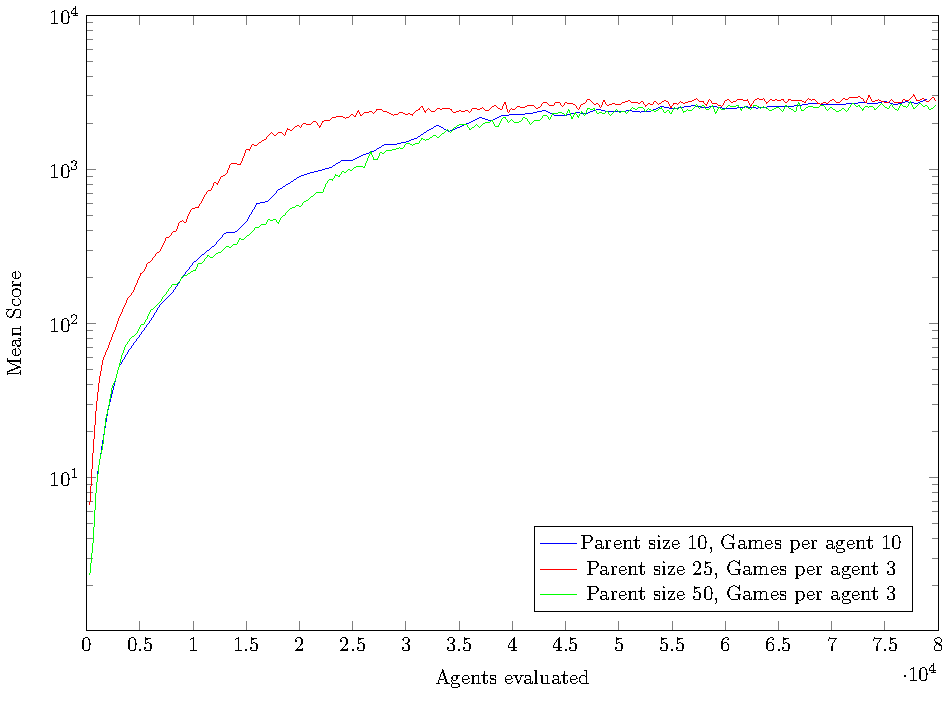
\includegraphics[scale=1]{data/ce_population_offspring/bestofeach_population/100x/PlotFile.pdf}
\caption{Best performing configurations for Population size 100}
\end{figure}

\clearpage

\begin{table}[H]
\centering
\small
\begin{tabular}{c c c r r r r}
Population & Parent & Games per Agent & mean & Q1 & Q2 & Q3\\
\hline
$200$ & $20$ & 1 & $2880.572$ & $2596.999$ & $2764.400$ & $3184.290$\\
$200$ & $50$ & 1 & $2950.767$ & $2564.118$ & $2841.065$ & $3377.189$\\
$200$ & $100$ & 1 & $2589.020$ & $2391.080$ & $2594.285$ & $2798.470$\\
\end{tabular}
\caption{Population 200 - The Cross-entropy method}
\end{table}

\begin{figure}[H]
\centering
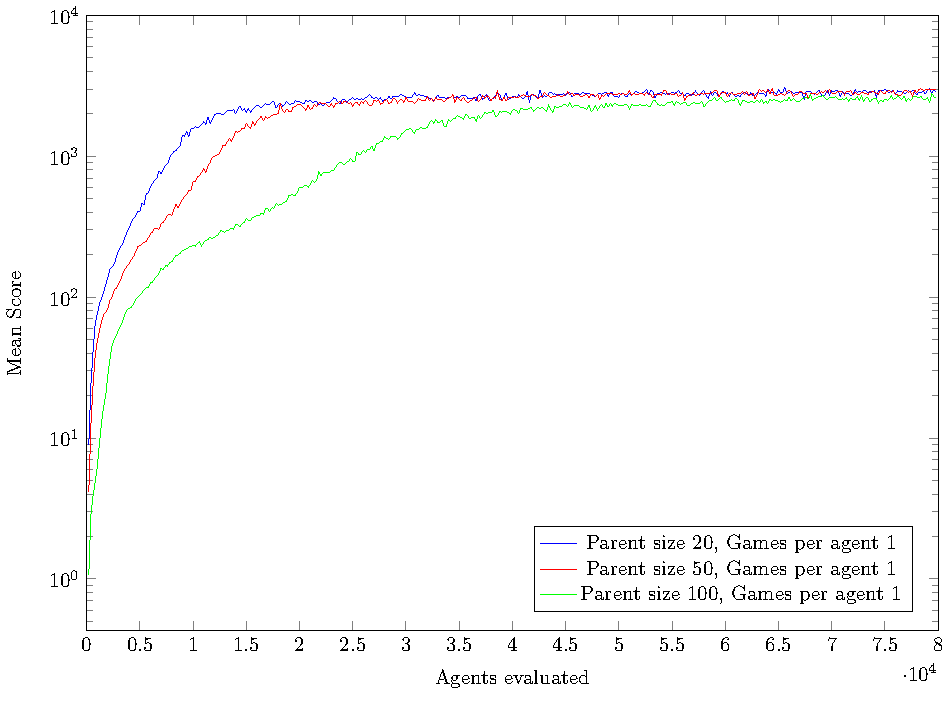
\includegraphics[scale=1]{data/ce_population_offspring/bestofeach_population/200x/PlotFile.pdf}
\caption{Best performing configurations for Population size 200}
\end{figure}

\clearpage

\begin{table}[H]
\centering
\small
\begin{tabular}{c c c r r r r}
Population & Parent & Games per Agent & mean & Q1 & Q2 & Q3\\
\hline
$13$ & $6$ & 7 & $2173.595$ & $1818.110$ & $2105.500$ & $2398.201$\\
$22$ & $5$ & 5 & $2371.793$ & $2013.168$ & $2412.815$ & $2708.931$\\
$50$ & $12$ & 5 & $2749.991$ & $2605.171$ & $2702.400$ & $2835.960$\\
$100$ & $25$ & 3 & $2776.560$ & $2397.691$ & $2742.950$ & $3027.541$\\
$200$ & $50$ & 1 & $2950.767$ & $2564.118$ & $2841.065$ & $3377.189$\\
\end{tabular}
\caption{Best configurations of all population sizes - Cross Entropy}
\end{table}

\begin{figure}[H]
\centering
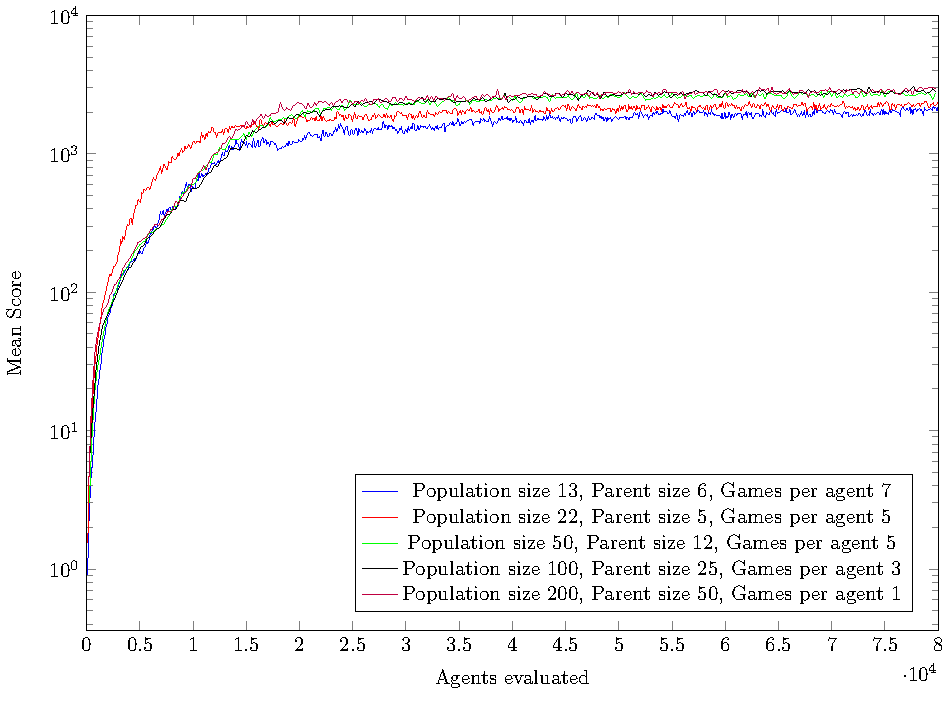
\includegraphics[scale=1]{data/ce_population_offspring/bestofall_population/PlotFile.pdf}
\caption{Best configurations of all Population sizes - The Cross-entropy method}
\end{figure}

\clearpage

\subsection{Optimal settings for CMA-ES - Initial Step-size \label{appendixCMAInitialSigma}}
Experiments to find the best performing initial Step-size for CMA-ES.

\begin{table}[h]
\centering
\begin{tabular}{l r}
Optimizer & CMA-ES\\
Number of Evaluations & 8000\\
Number of Learning Games &30\\
Population size& 13\\
Parent size & 6\\
Games per Agent & 1\\
Tetris Type & Normal\\
\hline
Recombination Type & Superlinear\\
Initial Sigma & See table \ref{InitialSigmaTest}
\end{tabular}
\caption{General setup for initial step-size experiments}
\end{table}

with the following initial sigma

\begin{table}[H]
\centering
\begin{tabular}{c | c c c c c c}
$\sigma_0$ & 0.1 & 0.2 & 0.5 & 0.8 & 1.0
\end{tabular}
\caption{Initial sigma configurations \label{InitialSigmaTest}}
\end{table}

\begin{tabular}{@{}l@{}l@{}}
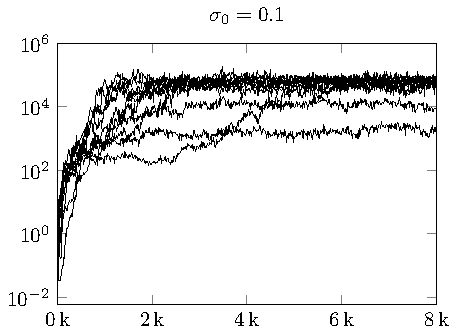
\includegraphics[scale=1]{plots/cma_initial_sigma_0_1} &
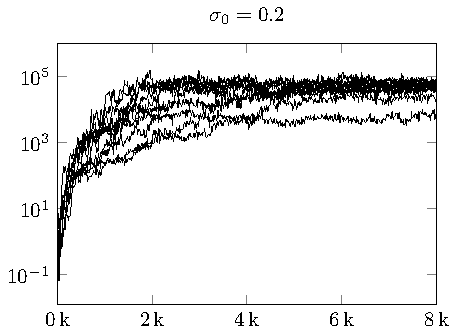
\includegraphics[scale=1]{plots/cma_initial_sigma_0_2}
\end{tabular}

\begin{tabular}{@{}l@{}l@{}}
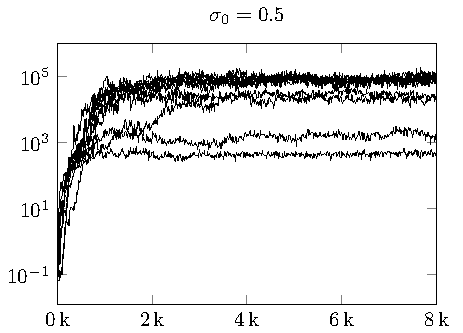
\includegraphics[scale=1]{plots/cma_initial_sigma_0_5} &
\includegraphics[scale=1]{plots/cma_initial_sigma_0_8}
\end{tabular}

\begin{tabular}{@{}l@{}l@{}}
\includegraphics[scale=1]{plots/cma_initial_sigma_1_0} &
\end{tabular}



\begin{figure}[H]
\centering
\begin{tabular}{r | r r r r r}
$\sigma_0$ & mean & Q1 & Q2 & Q3\\
\hline
0.1 & 50769.3 & 21301.1 & 54588.7 & 73972.4\\
0.2 & 42290.6 & 32180.2 & 42290.6 & 49337.4\\
0.5 & 53893.7 & 14211.1 & 66773.0 & 85816.7\\
0.8 & 37557.7 & 1422.8  & 15450.8 & 93719.4\\
1.0 & 49537.9 & 31369.8 & 49537.4 & 58454.6
\end{tabular}
\caption{Qualtile table with results of CMA-ES experiments regarding initial Step-size \label{CMAInitialSigmaConfigTestAppendix}}
\end{figure}


% initial Lower bound
\clearpage

\subsection{Optimal settings for CMA-ES - Lower bound \label{appendixCMALowerBound}}
Experiments to find the best performing lower bound of $\sigma \lambda_n > l$ for CMA-ES.

\begin{table}[h]
\centering
\begin{tabular}{l r}
Optimizer & CMA\\
Number of Evaluations & 8000\\
Number of Learning Games &30\\
Population size& 13\\
Parent size & 6\\
Games per Agent & 1\\
Tetris Type & Normal\\
\hline
Recombination Type & Superlinear\\
Lower bound & See table \ref{appendixLowerBound}
\end{tabular}
\caption{General setup for lower bound experiments}
\end{table}

with the following lower bounds

\begin{table}[H]
\centering
\begin{tabular}{c | c c c}
$l$ & 0.5 & 2.0 & 4.0
\end{tabular}
\caption{Lower bound configurations \label{appendixLowerBound}}
\end{table}
This sections lists the raw graphs of the experiments that were
to determine the effect of the initial sigma setting. 

\begin{tabular}{@{}l@{}l@{}}
\includegraphics[scale=1]{plots/cma_lower_bound_0_5} &
\includegraphics[scale=1]{plots/cma_lower_bound_2_0}\\
\includegraphics[scale=1]{plots/cma_lower_bound_4_0} &
\end{tabular}

\begin{figure}[H]
\centering
\begin{tabular}{r | r r r r r}
$l$ & mean & Q1 & Q2 & Q3\\
\hline
0.5 & 42800.7 & 6780.8  & 36863.0 & 74722.5\\
2.0 & 80733.4 & 62357.4 & 84349.0 & 108007.5\\
4.0 & 61497.2 & 55621.7 & 64940.1 & 81991.6\\
\end{tabular}
\caption{Results of CMA-ES lower bounds \label{appendixCMALowerBoundConfigTest}}
\end{figure}





\clearpage

\subsection{Optimal settings for CMA-ES - Experiment for finding the optimal settings \label{appendixCMAPopulationParent}}
Experiments finding the best performing configuration of Population/Parent size with
recombination type. The parent size is dependent on the recombination type, 
therefore these parameters are tested together.
\begin{table}[h]
\centering
\begin{tabular}{l r}
Optimizer & CMA\\
Number of Evaluations & 80000\\
Number of Learning Games &30\\
Population size& See table \ref{SuperCMAExperiment}\\
Parent size & See table \ref{SuperCMAExperiment}\\
Games per Agent & See table \ref{SuperCMAExperiment}\\
Tetris Type & Hard\\
\hline
Recombination Type & See table \ref{SuperCMAExperiment}\\
Initial Sigma & 1
\end{tabular}
\caption{CMA-ES experiment parameters for testing games per agent}
\end{table}

From the CMA-ES documentation tutorial \citep{hansen2011}, the Recombination Type dictates the Parent size.
However, we are also testing the Cross-entropy method Parent size for directly comparable
results. The Cross-entropy method uses $10 \% $ Parent size, therefore we will test all 
three Recombination types with this Parent size. This is in addition to the CMA-ES
documented $25 \% $ Parent size with equal Recombination and $50 \% $ Parent size for 
linear and superlinear recombination.

\begin{table}[H]
\centering
\begin{tabular}{c c l c}
Population Size & Parent size & Recombination Type & Games per Agent\\
\hline
$13$ & $1$ & EQUAL/LINEAR/SUPERLINEAR & 1/3/5/7/10\\
$13$ & $3$ & EQUAL & 1/3/5/7/10\\
$13$ & $6$ & LINEAR/SUPERLINEAR & 1/3/5/7/10\\
$22$ & $2$ & EQUAL/LINEAR/SUPERLINEAR & 1/3/5/7/10\\
$22$ & $5$ & EQUAL & 1/3/5/7/10\\
$22$ & $11$ & LINEAR/SUPERLINEAR & 1/3/5/7/10\\
$50$ & $5$ & EQUAL/LINEAR/SUPERLINEAR & 1/3/5/7/10\\
$50$ & $12$ & EQUAL & 1/3/5/7/10\\
$50$ & $25$ & LINEAR/SUPERLINEAR & 1/3/5/7/10\\
$100$ & $10$ & EQUAL/LINEAR/SUPERLINEAR & 1/3/5/7/10\\
$100$ & $25$ & EQUAL & 1/3/5/7/10\\
$100$ & $50$ & LINEAR/SUPERLINEAR & 1/3/5/7/10
\end{tabular}
\caption{Experiments overview with Parent size and according Recombination type and games per agent\label{SuperCMAExperimentAppendix}}
\end{table}


%\begin{figure}
%\centering
%\caption{Population size 12, Parent size 1, \\Meanscore of EQUAL recombination}
%\includegraphics[scale=0.5]{data/cma_population_offspring/12x_split/equal_l12_o1/mean/PlotFile.pdf}
%\end{figure}


\clearpage

\begin{figure}
	\centering
	\captionsetup[subfigure]{justification=centering}
    \begin{subfigure}[b]{0.49\textwidth}
    	\caption{Population size 13, Parent size 1,\\EQUAL recombination}
        \includegraphics[width=\textwidth]{data/cma_population_offspring/13x_split/equal_l13_o1/mean/PlotFile.pdf}
    \end{subfigure} 
    \begin{subfigure}[b]{0.49\textwidth}
    	\caption{Population size 13, Parent size 3,\\EQUAL recombination}
        \includegraphics[width=\textwidth]{data/cma_population_offspring/13x_split/equal_l13_o3/mean/PlotFile.pdf}
    \end{subfigure}
    \begin{subfigure}[b]{0.49\textwidth}
    	\caption{Population size 13, Parent size 1,\\LINEAR recombination}
        \includegraphics[width=\textwidth]{data/cma_population_offspring/13x_split/linear_l13_o1/mean/PlotFile.pdf}
    \end{subfigure}
    \begin{subfigure}[b]{0.49\textwidth}
    	\caption{Population size 13, Parent size 6,\\LINEAR recombination}
        \includegraphics[width=\textwidth]{data/cma_population_offspring/13x_split/linear_l13_o6/mean/PlotFile.pdf}
    \end{subfigure}
    \begin{subfigure}[b]{0.49\textwidth}
    	\caption{Population size 13, Parent size 1,\\SUPERLINEAR recombination}
        \includegraphics[width=\textwidth]{data/cma_population_offspring/13x_split/superlinear_l13_o1/mean/PlotFile.pdf}
    \end{subfigure}
    \begin{subfigure}[b]{0.49\textwidth}
    	\caption{Population size 13, Parent size 6,\\SUPERLINEAR recombination}
        \includegraphics[width=\textwidth]{data/cma_population_offspring/13x_split/superlinear_l13_o6/mean/PlotFile.pdf}
    \end{subfigure}
    
    \caption{Mean results for Population size 13 with variating Recombination type}
\end{figure}

\begin{figure}
    \centering
    \captionsetup[subfigure]{justification=centering}
    \begin{subfigure}[b]{0.49\textwidth}
    	\centering
        \caption{Population size 22, Parent size 2,\\EQUAL recombination}
        \includegraphics[width=\textwidth]{data/cma_population_offspring/22x_split/equal_l22_o2/mean/PlotFile.pdf}
    \end{subfigure} 
    \begin{subfigure}[b]{0.49\textwidth}
    	\centering
    	\caption{Population size 22, Parent size 5,\\EQUAL recombination}
        \includegraphics[width=\textwidth]{data/cma_population_offspring/22x_split/equal_l22_o5/mean/PlotFile.pdf}
    \end{subfigure}
    \begin{subfigure}[b]{0.49\textwidth}
    	\centering
    	\caption{Population size 22, Parent size 2,\\LINEAR recombination}
        \includegraphics[width=\textwidth]{data/cma_population_offspring/22x_split/linear_l22_o2/mean/PlotFile.pdf}
    \end{subfigure}
    \begin{subfigure}[b]{0.49\textwidth}
    	\centering
    	\caption{Population size 22, Parent size 11,\\LINEAR recombination}
        \includegraphics[width=\textwidth]{data/cma_population_offspring/22x_split/linear_l22_o11/mean/PlotFile.pdf}
    \end{subfigure}
    \begin{subfigure}[b]{0.49\textwidth}
    	\centering
    	\caption{Population size 22, Parent size 2,\\SUPERLINEAR recombination}
        \includegraphics[width=\textwidth]{data/cma_population_offspring/22x_split/superlinear_l22_o2/mean/PlotFile.pdf}
    \end{subfigure}
    \begin{subfigure}[b]{0.49\textwidth}
    	\centering
    	\caption{Population size 22, Parent size 11,\\SUPERLINEAR recombination}
        \includegraphics[width=\textwidth]{data/cma_population_offspring/22x_split/superlinear_l22_o11/mean/PlotFile.pdf}
    \end{subfigure}
    
    \caption{Mean results for Population size 22 with variating Recombination type}
\end{figure}

\begin{figure}
    \centering
    \captionsetup[subfigure]{justification=centering}
    \begin{subfigure}[b]{0.49\textwidth}
    	\centering
        \caption{Population size 50, Parent size 5,\\EQUAL recombination}
        \includegraphics[width=\textwidth]{data/cma_population_offspring/50x_split/equal_l50_o5/mean/PlotFile.pdf}
    \end{subfigure} 
    \begin{subfigure}[b]{0.49\textwidth}
    	\centering
    	\caption{Population size 50, Parent size 12,\\EQUAL recombination}
        \includegraphics[width=\textwidth]{data/cma_population_offspring/50x_split/equal_l50_o12/mean/PlotFile.pdf}
    \end{subfigure}
    \begin{subfigure}[b]{0.49\textwidth}
    	\centering
    	\caption{Population size 50, Parent size 5,\\LINEAR recombination}
        \includegraphics[width=\textwidth]{data/cma_population_offspring/50x_split/linear_l50_o5/mean/PlotFile.pdf}
    \end{subfigure}
    \begin{subfigure}[b]{0.49\textwidth}
    	\centering
    	\caption{Population size 50, Parent size 25,\\LINEAR recombination}
        \includegraphics[width=\textwidth]{data/cma_population_offspring/50x_split/linear_l50_o25/mean/PlotFile.pdf}
    \end{subfigure}
    \begin{subfigure}[b]{0.49\textwidth}
    	\centering
    	\caption{Population size 50, Parent size 5,\\SUPERLINEAR recombination}
        \includegraphics[width=\textwidth]{data/cma_population_offspring/50x_split/superlinear_l50_o5/mean/PlotFile.pdf}
    \end{subfigure}
    \begin{subfigure}[b]{0.49\textwidth}
    	\centering
    	\caption{Population size 50, Parent size 25,\\SUPERLINEAR recombination}
        \includegraphics[width=\textwidth]{data/cma_population_offspring/50x_split/superlinear_l50_o25/mean/PlotFile.pdf}
    \end{subfigure}
    
    \caption{Mean results for Population size 50 with variating Recombination type}
\end{figure}

\begin{figure}
    \centering
    \captionsetup[subfigure]{justification=centering}
    \begin{subfigure}[b]{0.49\textwidth}
    	\centering
        \caption{Population size 100, Parent size 10,\\EQUAL recombination}
        \includegraphics[width=\textwidth]{data/cma_population_offspring/100x_split/equal_l100_o10/mean/PlotFile.pdf}
    \end{subfigure} 
    \begin{subfigure}[b]{0.49\textwidth}
    	\centering
    	\caption{Population size 100, Parent size 25,\\EQUAL recombination}
        \includegraphics[width=\textwidth]{data/cma_population_offspring/100x_split/equal_l100_o25/mean/PlotFile.pdf}
    \end{subfigure}
    \begin{subfigure}[b]{0.49\textwidth}
    	\centering
    	\caption{Population size 100, Parent size 10,\\LINEAR recombination}
        \includegraphics[width=\textwidth]{data/cma_population_offspring/100x_split/linear_l100_o10/mean/PlotFile.pdf}
    \end{subfigure}
    \begin{subfigure}[b]{0.49\textwidth}
    	\centering
    	\caption{Population size 100, Parent size 50,\\LINEAR recombination}
        \includegraphics[width=\textwidth]{data/cma_population_offspring/100x_split/linear_l100_o50/mean/PlotFile.pdf}
    \end{subfigure}
    \begin{subfigure}[b]{0.49\textwidth}
    	\centering
    	\caption{Population size 100, Parent size 10,\\SUPERLINEAR recombination}
        \includegraphics[width=\textwidth]{data/cma_population_offspring/100x_split/superlinear_l100_o10/mean/PlotFile.pdf}
    \end{subfigure}
    \begin{subfigure}[b]{0.49\textwidth}
    	\centering
    	\caption{Population size 100, Parent size 50,\\SUPERLINEAR recombination}
        \includegraphics[width=\textwidth]{data/cma_population_offspring/100x_split/superlinear_l100_o50/mean/PlotFile.pdf}
    \end{subfigure}
    
    \caption{Mean results for Population size 100 with variating Recombination type}
\end{figure}

\clearpage

%\comment{Will be swapped}
%\begin{table}[H]
%\centering
%\small
%\begin{tabular}{c c c c r r r r}
%Population & Parent & Recombination & Games per Agent & mean & Q1 & Q2 & Q3\\
%\hline
%$13$ & $1$ & EQUAL & 1 & $86.998$ & $53.557$ & $63.417$ & $111.313$\\
%$13$ & $1$ & EQUAL & 3 & $458.616$ & $256.637$ & $349.033$ & $576.899$\\
%$13$ & $1$ & EQUAL & 5 & $1089.245$ & $850.220$ & $1104.535$ & $1299.039$\\
%$13$ & $1$ & EQUAL & 7 & $1081.248$ & $918.049$ & $1089.400$ & $1248.619$\\
%\hdashline
%$13$ & $1$ & EQUAL & 10 & $1134.339$ & $863.523$ & $1061.050$ & $1297.359$\\
%\hdashline
%$13$ & $1$ & LINEAR & 1 & $76.228$ & $45.587$ & $53.917$ & $74.353$\\
%$13$ & $1$ & LINEAR & 3 & $717.883$ & $380.890$ & $556.950$ & $878.597$\\
%$13$ & $1$ & LINEAR & 5 & $720.393$ & $503.130$ & $708.484$ & $893.517$\\
%$13$ & $1$ & LINEAR & 7 & $1043.547$ & $732.367$ & $969.217$ & $1234.040$\\
%\hdashline
%$13$ & $1$ & LINEAR & 10 & $1276.041$ & $1135.609$ & $1196.120$ & $1502.029$\\
%\hdashline
%$13$ & $1$ & SUPERLINEAR & 1 & $64.211$ & $45.687$ & $64.483$ & $78.090$\\
%$13$ & $1$ & SUPERLINEAR & 3 & $646.760$ & $429.043$ & $661.817$ & $860.470$\\
%$13$ & $1$ & SUPERLINEAR & 5 & $925.410$ & $726.360$ & $948.300$ & $1158.021$\\
%$13$ & $1$ & SUPERLINEAR & 7 & $1034.002$ & $792.567$ & $924.350$ & $1269.131$\\
%\hdashline
%$13$ & $1$ & SUPERLINEAR & 10 & $1401.300$ & $1194.430$ & $1440.500$ & $1569.012$\\
%\hdashline
%\end{tabular}
%\caption{Population size 13, Parent size 1 - "The Cross-entropy method"-inspired configuration}
%\end{table}

\begin{table}[H]
\centering
\small
\begin{tabular}{c c c c r r r r}
Population & Parent & Recombination & Games per Agent & mean & Q1 & Q2 & Q3\\
\hline
$13$ & $1$ & EQUAL & 1 & $91.077$ & $47.463$ & $67.483$ & $114.117$\\
$13$ & $1$ & EQUAL & 3 & $615.599$ & $367.963$ & $497.700$ & $764.380$\\
$13$ & $1$ & EQUAL & 5 & $922.903$ & $725.477$ & $977.217$ & $1092.980$\\
$13$ & $1$ & EQUAL & 7 & $1046.058$ & $904.673$ & $1117.800$ & $1262.589$\\
\hdashline
$13$ & $1$ & EQUAL & 10 & $1372.659$ & $1178.270$ & $1341.850$ & $1502.669$\\
\hdashline
$13$ & $1$ & LINEAR & 1 & $79.406$ & $43.650$ & $60.750$ & $87.883$\\
$13$ & $1$ & LINEAR & 3 & $578.311$ & $370.437$ & $553.917$ & $726.220$\\
$13$ & $1$ & LINEAR & 5 & $997.244$ & $764.243$ & $908.317$ & $1252.890$\\
$13$ & $1$ & LINEAR & 7 & $1107.305$ & $866.360$ & $1200.465$ & $1270.728$\\
\hdashline
$13$ & $1$ & LINEAR & 10 & $1315.537$ & $1081.220$ & $1313.470$ & $1437.808$\\
\hdashline
$13$ & $1$ & SUPERLINEAR & 1 & $81.547$ & $59.697$ & $71.517$ & $83.883$\\
$13$ & $1$ & SUPERLINEAR & 3 & $613.279$ & $270.957$ & $602.417$ & $812.003$\\
$13$ & $1$ & SUPERLINEAR & 5 & $909.034$ & $595.153$ & $789.684$ & $1186.589$\\
$13$ & $1$ & SUPERLINEAR & 7 & $1109.016$ & $891.820$ & $1110.300$ & $1369.321$\\
\hdashline
$13$ & $1$ & SUPERLINEAR & 10 & $1251.003$ & $939.580$ & $1196.170$ & $1438.529$\\
\hdashline
\end{tabular}
\caption{Population size 13, Parent size 1 - "The Cross-entropy method-inspired" configuration}
\end{table}

%\begin{table}[H]
%\centering
%\small
%\begin{tabular}{c c c c r r r r}
%Population & Parent & Recombination & Games per Agent & mean & Q1 & Q2 & Q3\\
%\hline
%$12$ & $3$ & EQUAL & 1 & $461.762$ & $266.047$ & $408.034$ & $639.013$\\
%$12$ & $3$ & EQUAL & 3 & $1364.176$ & $1199.310$ & $1438.880$ & $1579.560$\\
%$12$ & $3$ & EQUAL & 5 & $1754.634$ & $1464.239$ & $1621.035$ & $1945.010$\\
%$12$ & $3$ & EQUAL & 7 & $1884.765$ & $1614.661$ & $1800.485$ & $2156.972$\\
%\hdashline
%$12$ & $3$ & EQUAL & 10 & $1940.783$ & $1566.721$ & $1913.415$ & $2210.251$\\
%\hdashline
%$12$ & $6$ & LINEAR & 1 & $626.867$ & $447.440$ & $538.150$ & $724.913$\\
%$12$ & $6$ & LINEAR & 3 & $1844.453$ & $1568.829$ & $1831.265$ & $2227.479$\\
%$12$ & $6$ & LINEAR & 5 & $2148.853$ & $1846.459$ & $2118.335$ & $2588.010$\\
%$12$ & $6$ & LINEAR & 7 & $2144.345$ & $1860.340$ & $2160.900$ & $2428.348$\\
%\hdashline
%$12$ & $6$ & LINEAR & 10 & $2365.089$ & $2072.719$ & $2263.665$ & $2637.732$\\
%\hdashline
%$12$ & $6$ & SUPERLINEAR & 1 & $669.005$ & $506.817$ & $648.167$ & $836.377$\\
%$12$ & $6$ & SUPERLINEAR & 3 & $1901.814$ & $1572.260$ & $1932.515$ & $2151.189$\\
%$12$ & $6$ & SUPERLINEAR & 5 & $2098.654$ & $1965.472$ & $2115.250$ & $2453.069$\\
%$12$ & $6$ & SUPERLINEAR & 7 & $2402.888$ & $2055.329$ & $2387.700$ & $2635.870$\\
%\hdashline
%$12$ & $6$ & SUPERLINEAR & 10 & $2472.293$ & $2194.049$ & $2430.780$ & $2709.040$\\
%\hdashline
%\end{tabular}
%\caption{Population size 13, Parent size 3/6 - CMA-ES configuration}
%\end{table}

\begin{table}[H]
\centering
\small
\begin{tabular}{c c c c r r r r}
Population & Parent & Recombination & Games per Agent & mean & Q1 & Q2 & Q3\\
\hline
$13$ & $3$ & EQUAL & 1 & $497.271$ & $286.093$ & $378.983$ & $592.170$\\
$13$ & $3$ & EQUAL & 3 & $1361.406$ & $1131.579$ & $1343.515$ & $1671.548$\\
$13$ & $3$ & EQUAL & 5 & $1679.227$ & $1417.910$ & $1644.900$ & $1831.780$\\
$13$ & $3$ & EQUAL & 7 & $1865.261$ & $1474.159$ & $1755.880$ & $2074.619$\\
\hdashline
$13$ & $3$ & EQUAL & 10 & $2035.384$ & $1855.050$ & $2054.114$ & $2275.999$\\
\hdashline
$13$ & $6$ & LINEAR & 1 & $710.275$ & $487.112$ & $628.884$ & $940.673$\\
$13$ & $6$ & LINEAR & 3 & $1939.206$ & $1691.011$ & $1932.685$ & $2153.378$\\
$13$ & $6$ & LINEAR & 5 & $2194.410$ & $1981.779$ & $2277.280$ & $2432.470$\\
$13$ & $6$ & LINEAR & 7 & $2120.762$ & $2090.310$ & $2302.350$ & $2392.740$\\
\hdashline
$13$ & $6$ & LINEAR & 10 & $2304.402$ & $2196.891$ & $2371.700$ & $2698.631$\\
\hdashline
$13$ & $6$ & SUPERLINEAR & 1 & $914.616$ & $575.833$ & $925.200$ & $1176.779$\\
$13$ & $6$ & SUPERLINEAR & 3 & $1838.479$ & $1570.490$ & $1792.185$ & $1955.269$\\
$13$ & $6$ & SUPERLINEAR & 5 & $1986.118$ & $1757.779$ & $1914.700$ & $2280.298$\\
$13$ & $6$ & SUPERLINEAR & 7 & $2351.788$ & $2138.170$ & $2299.835$ & $2498.131$\\
\hdashline
$13$ & $6$ & SUPERLINEAR & 10 & $2495.021$ & $2182.641$ & $2512.720$ & $2887.450$\\
\hdashline
\end{tabular}
\caption{Population size 13, Parent size 3/6 - CMA-ES configuration}
\end{table}


\begin{table}[H]
\centering
\small
\begin{tabular}{c c c c r r r r}
Population & Parent & Recombination & Games per Agent & mean & Q1 & Q2 & Q3\\
\hline
$22$ & $2$ & EQUAL & 1 & $684.551$ & $429.890$ & $597.534$ & $877.150$\\
$22$ & $2$ & EQUAL & 3 & $1473.504$ & $1197.290$ & $1490.865$ & $1713.091$\\
$22$ & $2$ & EQUAL & 5 & $1648.777$ & $1425.150$ & $1630.535$ & $1826.372$\\
$22$ & $2$ & EQUAL & 7 & $1762.786$ & $1521.832$ & $1769.180$ & $2033.799$\\
\hdashline
$22$ & $2$ & EQUAL & 10 & $1895.305$ & $1630.891$ & $1849.75$ & $2043.442$\\
\hdashline
$22$ & $2$ & LINEAR & 1 & $513.271$ & $398.023$ & $524.850$ & $589.467$\\
$22$ & $2$ & LINEAR & 3 & $1374.423$ & $1082.859$ & $1255.985$ & $1561.119$\\
$22$ & $2$ & LINEAR & 5 & $1607.568$ & $1513.389$ & $1656.465$ & $1791.069$\\
$22$ & $2$ & LINEAR & 7 & $1770.294$ & $1538.900$ & $1691.165$ & $1881.590$\\
\hdashline
$22$ & $2$ & LINEAR & 10 & $2158.396$ & $1966.351$ & $2085.235$ & $2162.541$\\
\hdashline
$22$ & $2$ & SUPERLINEAR & 1 & $698.811$ & $359.367$ & $622.467$ & $937.423$\\
$22$ & $2$ & SUPERLINEAR & 3 & $1447.704$ & $1281.119$ & $1452.680$ & $1640.468$\\
$22$ & $2$ & SUPERLINEAR & 5 & $1714.875$ & $1362.931$ & $1733.230$ & $2023.590$\\
\hdashline
$22$ & $2$ & SUPERLINEAR & 7 & $1783.623$ & $1603.389$ & $1720.335$ & $1937.749$\\
\hdashline
$22$ & $2$ & SUPERLINEAR & 10 & $1859.642$ & $1636.870$ & $1915.650$ & $2208.830$\\
\end{tabular}
\caption{Population size 22, Parent size 2 - "The Cross-entropy method-inspired" configuration}
\end{table}


\begin{table}[H]
\centering
\small
\begin{tabular}{c c c c r r r r}
Population & Parent & Recombination & Games per Agent & mean & Q1 & Q2 & Q3\\
\hline
$22$ & $5$ & EQUAL & 1 & $1411.458$ & $1207.060$ & $1528.050$ & $1707.590$\\
$22$ & $5$ & EQUAL & 3 & $2209.730$ & $2129.521$ & $2213.285$ & $2471.751$\\
$22$ & $5$ & EQUAL & 5 & $2274.419$ & $1933.249$ & $2187.800$ & $2570.399$\\
$22$ & $5$ & EQUAL & 7 & $2386.088$ & $2112.841$ & $2328.500$ & $2573.261$\\
\hdashline
$22$ & $5$ & EQUAL & 10 & $2462.409$ & $2277.180$ & $2418.100$ & $2600.411$\\
\hdashline
$22$ & $11$ & LINEAR & 1 & $1604.434$ & $1181.603$ & $1549.735$ & $1678.111$\\
$22$ & $11$ & LINEAR & 3 & $2774.378$ & $2460.992$ & $2594.900$ & $3030.310$\\
$22$ & $11$ & LINEAR & 5 & $2530.796$ & $2382.050$ & $2658.915$ & $2990.851$\\
\hdashline
$22$ & $11$ & LINEAR & 7 & $2763.353$ & $2597.450$ & $2705.080$ & $3000.242$\\
\hdashline
$22$ & $11$ & LINEAR & 10 & $2707.983$ & $2146.209$ & $2800.435$ & $3273.401$\\
$22$ & $11$ & SUPERLINEAR & 1 & $1666.214$ & $1447.430$ & $1660.900$ & $1856.908$\\
$22$ & $11$ & SUPERLINEAR & 3 & $2581.119$ & $2306.02$ & $2548.380$ & $2759.428$\\
$22$ & $11$ & SUPERLINEAR & 5 & $2635.429$ & $2409.620$ & $2574.785$ & $2863.849$\\
$22$ & $11$ & SUPERLINEAR & 7 & $2661.638$ & $2411.232$ & $2575.030$ & $2945.200$\\
\hdashline
$22$ & $11$ & SUPERLINEAR & 10 & $2849.220$ & $2500.231$ & $2835.450$ & $3143.121$\\
\hdashline
\end{tabular}
\caption{Population size 22, Parent size 5/11 - CMA-ES configuration}
\end{table}


\begin{table}[H]
\centering
\small
\begin{tabular}{c c c c r r r r}
Population & Parent & Recombination & Games per Agent & mean & Q1 & Q2 & Q3\\
\hline
$50$ & $5$ & EQUAL & 1 & $1999.620$ & $1789.150$ & $1902.020$ & $2161.948$\\
$50$ & $5$ & EQUAL & 3 & $2471.173$ & $2178.651$ & $2389.070$ & $2660.220$\\
$50$ & $5$ & EQUAL & 5 & $2849.482$ & $2459.460$ & $2875.835$ & $3276.190$\\
$50$ & $5$ & EQUAL & 7 & $2466.801$ & $2355.349$ & $2517.335$ & $2644.751$\\
\hdashline
$50$ & $5$ & EQUAL & 10 & $2801.923$ & $2479.088$ & $2915.980$ & $3081.018$\\
\hdashline
$50$ & $5$ & LINEAR & 1 & $1931.703$ & $1659.412$ & $1885.150$ & $2130.479$\\
$50$ & $5$ & LINEAR & 3 & $2612.345$ & $2380.759$ & $2529.150$ & $2796.729$\\
$50$ & $5$ & LINEAR & 5 & $2410.633$ & $2067.111$ & $2357.830$ & $2675.572$\\
\hdashline
$50$ & $5$ & LINEAR & 7 & $2842.090$ & $2497.952$ & $2922.965$ & $3136.509$\\
\hdashline
$50$ & $5$ & LINEAR & 10 & $2696.952$ & $2518.290$ & $2678.400$ & $2923.010$\\
$50$ & $5$ & SUPERLINEAR & 1 & $1962.410$ & $1715.568$ & $1781.865$ & $2009.488$\\
$50$ & $5$ & SUPERLINEAR & 3 & $2493.884$ & $2220.200$ & $2398.230$ & $2762.609$\\
$50$ & $5$ & SUPERLINEAR & 5 & $2541.065$ & $2268.881$ & $2593.150$ & $2974.558$\\
$50$ & $5$ & SUPERLINEAR & 7 & $2647.412$ & $2448.010$ & $2745.400$ & $3058.870$\\
\hdashline
$50$ & $5$ & SUPERLINEAR & 10 & $2757.388$ & $2357.062$ & $2886.950$ & $3187.282$\\
\hdashline
\end{tabular}
\caption{Population size 50, Parent size 5 - "The Cross-entropy method-inspired" configuration}
\end{table}

\begin{table}[H]
\centering
\small
\begin{tabular}{c c c c r r r r}
Population & Parent & Recombination & Games per Agent & mean & Q1 & Q2 & Q3\\
\hline
$50$ & $12$ & EQUAL & 1 & $2395.091$ & $2095.030$ & $2442.485$ & $2778.160$\\
$50$ & $12$ & EQUAL & 3 & $2878.667$ & $2550.399$ & $2794.915$ & $3102.639$\\
$50$ & $12$ & EQUAL & 5 & $2760.846$ & $2509.000$ & $2695.450$ & $3006.988$\\
$50$ & $12$ & EQUAL & 7 & $2913.846$ & $2627.310$ & $2809.600$ & $3128.439$\\
\hdashline
$50$ & $12$ & EQUAL & 10 & $2957.794$ & $2636.478$ & $2843.380$ & $3222.420$\\
\hdashline
$50$ & $25$ & LINEAR & 1 & $2355.564$ & $2262.991$ & $2543.665$ & $2752.431$\\
$50$ & $25$ & LINEAR & 3 & $2857.170$ & $2464.251$ & $2830.765$ & $3209.929$\\
$50$ & $25$ & LINEAR & 5 & $3036.881$ & $2807.050$ & $3095.300$ & $3416.750$\\
$50$ & $25$ & LINEAR & 7 & $3043.399$ & $2821.049$ & $3099.235$ & $3239.032$\\
\hdashline
$50$ & $25$ & LINEAR & 10 & $3167.873$ & $2941.590$ & $3130.385$ & $3415.520$\\
\hdashline
$50$ & $25$ & SUPERLINEAR & 1 & $2418.057$ & $2352.851$ & $2553.465$ & $2718.759$\\
$50$ & $25$ & SUPERLINEAR & 3 & $2958.686$ & $2715.579$ & $2941.800$ & $3173.361$\\
\hdashline
$50$ & $25$ & SUPERLINEAR & 5 & $3211.658$ & $2889.689$ & $3305.485$ & $3694.480$\\
\hdashline
$50$ & $25$ & SUPERLINEAR & 7 & $3147.611$ & $2799.510$ & $3123.550$ & $3457.999$\\
$50$ & $25$ & SUPERLINEAR & 10 & $3265.516$ & $2928.771$ & $3162.250$ & $3389.121$\\
\end{tabular}
\caption{Population size 50, Parent size 12/25 - CMA-ES configuration}
\end{table}


\begin{table}[H]
\centering
\small
\begin{tabular}{c c c c r r r r}
Population & Parent & Recombination & Games per Agent & mean & Q1 & Q2 & Q3\\
\hline
$100$ & $10$ & EQUAL & 1 & $2528.158$ & $2380.122$ & $2680.785$ & $2782.850$\\
$100$ & $10$ & EQUAL & 3 & $2763.118$ & $2488.878$ & $2696.685$ & $2962.190$\\
$100$ & $10$ & EQUAL & 5 & $2783.246$ & $2399.949$ & $2693.285$ & $2900.391$\\
\hdashline
$100$ & $10$ & EQUAL & 7 & $3016.342$ & $2835.049$ & $2985.150$ & $3292.910$\\
\hdashline
$100$ & $10$ & EQUAL & 10 & $2940.037$ & $2703.859$ & $2920.615$ & $3216.410$\\
$100$ & $10$ & LINEAR & 1 & $2655.099$ & $2409.162$ & $2691.850$ & $2961.091$\\
$100$ & $10$ & LINEAR & 3 & $2823.674$ & $2526.560$ & $2792.500$ & $2974.549$\\
\hdashline
$100$ & $10$ & LINEAR & 5 & $3204.395$ & $2928.050$ & $3248.515$ & $3371.008$\\
\hdashline
$100$ & $10$ & LINEAR & 7 & $2993.126$ & $2639.021$ & $3031.065$ & $3277.642$\\
$100$ & $10$ & LINEAR & 10 & $2726.273$ & $2402.502$ & $2748.535$ & $3009.198$\\
$100$ & $10$ & SUPERLINEAR & 1 & $2571.936$ & $2211.051$ & $2634.850$ & $2811.190$\\
$100$ & $10$ & SUPERLINEAR & 3 & $2853.959$ & $2552.749$ & $2870.600$ & $3005.292$\\
\hdashline
$100$ & $10$ & SUPERLINEAR & 5 & $3009.495$ & $2816.660$ & $2989.900$ & $3189.310$\\
\hdashline
$100$ & $10$ & SUPERLINEAR & 7 & $2935.614$ & $2540.342$ & $2887.085$ & $3232.508$\\
$100$ & $10$ & SUPERLINEAR & 10 & $2941.535$ & $2705.290$ & $2893.580$ & $3153.510$\\
\end{tabular}
\caption{Population size 100, Parent size 10 - "The Cross-entropy method-inspired" configuration}
\end{table}


\begin{table}[H]
\centering
\small
\begin{tabular}{c c c c r r r r}
Population & Parent & Recombination & Games per Agent & mean & Q1 & Q2 & Q3\\
\hline
$100$ & $25$ & EQUAL & 1 & $2885.131$ & $2565.572$ & $2886.735$ & $3231.600$\\
\hdashline
$100$ & $25$ & EQUAL & 3 & $3244.544$ & $2924.488$ & $3270.885$ & $3525.671$\\
\hdashline
$100$ & $25$ & EQUAL & 5 & $3065.143$ & $2773.848$ & $3032.830$ & $3347.358$\\
$100$ & $25$ & EQUAL & 7 & $3125.085$ & $2758.298$ & $3054.950$ & $3486.672$\\
$100$ & $25$ & EQUAL & 10 & $3258.533$ & $2976.271$ & $3144.750$ & $3598.868$\\
$100$ & $50$ & LINEAR & 1 & $3099.651$ & $2814.781$ & $3019.830$ & $3466.380$\\
$100$ & $50$ & LINEAR & 3 & $3125.019$ & $2706.618$ & $3087.815$ & $3368.681$\\
$100$ & $50$ & LINEAR & 5 & $3171.761$ & $2941.030$ & $3138.515$ & $3436.670$\\
\hdashline
$100$ & $50$ & LINEAR & 7 & $3322.076$ & $3160.098$ & $3289.370$ & $3537.850$\\
\hdashline
$100$ & $50$ & LINEAR & 10 & $3320.153$ & $3040.611$ & $3291.335$ & $3633.491$\\
$100$ & $50$ & SUPERLINEAR & 1 & $3162.245$ & $2815.099$ & $3093.050$ & $3482.748$\\
$100$ & $50$ & SUPERLINEAR & 3 & $3188.324$ & $2781.382$ & $3258.400$ & $3413.710$\\
\hdashline
$100$ & $50$ & SUPERLINEAR & 5 & $3304.119$ & $3004.140$ & $3226.235$ & $3679.359$\\
\hdashline
$100$ & $50$ & SUPERLINEAR & 7 & $3072.331$ & $2682.300$ & $2964.850$ & $3403.132$\\
$100$ & $50$ & SUPERLINEAR & 10 & $3106.917$ & $2914.349$ & $3162.250$ & $3324.970$\\
\end{tabular}
\caption{Population size 100, Parent size 25/50 - CMA-ES configuration}
\end{table}

\clearpage

%\begin{table}[H]
%\centering
%\small
%\begin{tabular}{c c c c r r r r}
%Population & Parent & Recombination & Games per Agent & mean & Q1 & Q2 & Q3\\
%\hline
%$13$ & $1$ & EQUAL & 10 & $1134.339$ & $863.523$ & $1061.050$ & $1297.359$\\
%$13$ & $1$ & LINEAR & 10 & $1276.041$ & $1135.609$ & $1196.120$ & $1502.029$\\
%$13$ & $1$ & SUPERLINEAR & 10 & $1401.300$ & $1194.430$ & $1440.500$ & $1569.012$\\
%$13$ & $3$ & EQUAL & 10 & $1940.783$ & $1566.721$ & $1913.415$ & $2210.251$\\
%$13$ & $6$ & LINEAR & 10 & $2365.089$ & $2072.719$ & $2263.665$ & $2637.732$\\
%$13$ & $6$ & SUPERLINEAR & 10 & $2472.293$ & $2194.049$ & $2430.780$ & $2709.040$\\
%\end{tabular}
%\caption{Best performing configurations for Population size 13}
%\end{table}

\begin{table}[H]
\centering
\small
\begin{tabular}{c c c c r r r r}
Population & Parent & Recombination & Games per Agent & mean & Q1 & Q2 & Q3\\
\hline
$13$ & $1$ & EQUAL & 10 & $1372.659$ & $1178.270$ & $1341.850$ & $1502.669$\\
$13$ & $1$ & LINEAR & 10 & $1315.537$ & $1081.220$ & $1313.470$ & $1437.808$\\
$13$ & $1$ & SUPERLINEAR & 10 & $1251.003$ & $939.580$ & $1196.170$ & $1438.529$\\
$13$ & $3$ & EQUAL & 10 & $2035.384$ & $1855.050$ & $2054.114$ & $2275.999$\\
$13$ & $6$ & LINEAR & 10 & $2304.402$ & $2196.891$ & $2371.700$ & $2698.631$\\
$13$ & $6$ & SUPERLINEAR & 10 & $2495.021$ & $2182.641$ & $2512.720$ & $2887.450$\\
\end{tabular}
\caption{Best performing configurations for Population size 13}
\end{table}

\begin{figure}[H]
\centering
\includegraphics[scale=1]{data/cma_population_offspring/bestofeach_population/13x/PlotFile.pdf}
\caption{Best performing configurations for Population size 13}
\end{figure}

\clearpage

\begin{table}[H]
\centering
\small
\begin{tabular}{c c c c r r r r}
Population & Parent & Recombination & Games per Agent & mean & Q1 & Q2 & Q3\\
\hline
$22$ & $2$ & EQUAL & 10 & $1895.305$ & $1630.891$ & $1849.75$ & $2043.442$\\
$22$ & $2$ & LINEAR & 10 & $2158.396$ & $1966.351$ & $2085.235$ & $2162.541$\\
$22$ & $2$ & SUPERLINEAR & 7 & $1783.623$ & $1603.389$ & $1720.335$ & $1937.749$\\
$22$ & $5$ & EQUAL & 10 & $2462.409$ & $2277.180$ & $2418.100$ & $2600.411$\\
$22$ & $11$ & LINEAR & 7 & $2763.353$ & $2597.450$ & $2705.080$ & $3000.242$\\
$22$ & $11$ & SUPERLINEAR & 10 & $2849.220$ & $2500.231$ & $2835.450$ & $3143.121$\\
\end{tabular}
\caption{Best performing configurations for Population size 22}
\end{table}

\begin{figure}[H]
\centering
\includegraphics[scale=1]{data/cma_population_offspring/bestofeach_population/22x/PlotFile.pdf}
\caption{Best performing configurations for Population size 22}
\end{figure}

\clearpage

\begin{table}[H]
\centering
\small
\begin{tabular}{c c c c r r r r}
Population & Parent & Recombination & Games per Agent & mean & Q1 & Q2 & Q3\\
\hline
$50$ & $5$ & EQUAL & 10 & $2801.923$ & $2479.088$ & $2915.980$ & $3081.018$\\
$50$ & $5$ & LINEAR & 7 & $2842.090$ & $2497.952$ & $2922.965$ & $3136.509$\\
$50$ & $5$ & SUPERLINEAR & 10 & $2757.388$ & $2357.062$ & $2886.950$ & $3187.282$\\
$50$ & $12$ & EQUAL & 10 & $2957.794$ & $2636.478$ & $2843.380$ & $3222.420$\\
$50$ & $25$ & LINEAR & 10 & $3167.873$ & $2941.590$ & $3130.385$ & $3415.520$\\
$50$ & $25$ & SUPERLINEAR & 5 & $3211.658$ & $2889.689$ & $3305.485$ & $3694.480$\\
\end{tabular}
\caption{Best performing configurations for Population size 50}
\end{table}

\begin{figure}[H]
\centering
\includegraphics[scale=1]{data/cma_population_offspring/bestofeach_population/50x/PlotFile.pdf}
\caption{Best performing configurations for Population size 50}
\end{figure}

\clearpage

\begin{table}[H]
\centering
\small
\begin{tabular}{c c c c r r r r}
Population & Parent & Recombination & Games per Agent & mean & Q1 & Q2 & Q3\\
\hline
$100$ & $10$ & EQUAL & 7 & $3016.342$ & $2835.049$ & $2985.150$ & $3292.910$\\
$100$ & $10$ & LINEAR & 5 & $3204.395$ & $2928.050$ & $3248.515$ & $3371.008$\\
$100$ & $10$ & SUPERLINEAR & 5 & $3009.495$ & $2816.660$ & $2989.900$ & $3189.310$\\
$100$ & $25$ & EQUAL & 3 & $3244.544$ & $2924.488$ & $3270.885$ & $3525.671$\\
$100$ & $50$ & LINEAR & 7 & $3322.076$ & $3160.098$ & $3289.370$ & $3537.850$\\
$100$ & $50$ & SUPERLINEAR & 5 & $3304.119$ & $3004.140$ & $3226.235$ & $3679.359$\\
\end{tabular}
\caption{Best performing configurations for Population size 100}
\end{table}

\begin{figure}[H]
\centering
\includegraphics[scale=1]{data/cma_population_offspring/bestofeach_population/100x/PlotFile.pdf}
\caption{Best performing configurations for Population size 100}
\end{figure}

\clearpage 

\begin{table}[H]
\centering
\small
\begin{tabular}{c c c c r r r r}
Population & Parent & Recombination & Games per Agent & mean & Q1 & Q2 & Q3\\
\hline
$13$ & $6$ & SUPERLINEAR & 10 & $2495.021$ & $2182.641$ & $2512.720$ & $2887.450$\\
$22$ & $11$ & SUPERLINEAR & 10 & $2849.220$ & $2500.231$ & $2835.450$ & $3143.121$\\
$50$ & $25$ & SUPERLINEAR & 5 & $3211.658$ & $2889.689$ & $3305.485$ & $3694.480$\\
$100$ & $50$ & LINEAR & 7 & $3322.076$ & $3160.098$ & $3289.370$ & $3537.850$\\
\end{tabular}
\caption{Best performing configurations of all Population sizes}
\end{table}

\begin{figure}[H]
\centering
\includegraphics[scale=1]{data/cma_population_offspring/bestofall_population/PlotFile.pdf}
\caption{Best performing configurations of all Population sizes}
\end{figure}



\clearpage

\subsection{Comparison - Initial comparison}
Comparison between the verified Cross-entropy method and Shark \citep{shark08} default settings CMA-ES.

\begin{table}[h]
\centering
\small
\begin{tabular}{l r}
Optimizer & CMA\\
Number of Evaluations & 8000\\
Number of Learning Games & 30\\
Population size& 13\\
Parent size & 6\\
Games per Agent & 1\\
Tetris Type & Normal\\
\hline
Recombination Type & Superlinear\\
Initial Sigma & $\frac{1}{\sqrt{22}}$\\
\quad & \quad
\end{tabular}
\quad
\begin{tabular}{l r}
Optimizer & Cross Entropy\\
Number of Evaluations & 8000\\
Number of Learning Games & 30\\
Population size & 100\\
Parent size & 10\\
Games per Agent & 1\\
Tetris Type & Normal\\
\hline
Sigma & 100\\
Noise Type & Constant\\
Noise & 4
\end{tabular}
\caption{Shark default settings CMA-ES and the verified Cross-entropy method}
\end{table}

\begin{figure}[H]
\begin{tabular}{@{}c@{}c@{}}
CMA-ES & The Cross-entropy method\\
\includegraphics[scale=1]{plots/cma_initial_sigma_0_5} &
\includegraphics[scale=1]{plots/ce_ConstantNoise_l100_o10_all}
\end{tabular}
\caption{10 experiments with default settings Cross-entropy method (From papers) and CMA-ES (From Shark) \label{fig:appendix:initialNonmean}}
\end{figure}

\begin{figure}[H]
\begin{center}
\includegraphics[scale=0.8]{plots/cmaCePlot}
\end{center}
\caption{Initial comparison between CMA-ES and the Cross-entropy method \label{fig:appendixCMA_VS_CE_00}}
\end{figure}

\clearpage

\subsection{Comparison - Optimized settings}
Final comparison experiment using the optimized settings determined experimentally 
in the sections \ref{optimalsettingsce} for the Cross-entropy method 
and \ref{optimalsettingscma} for CMA-ES.

\begin{table}[H]
\centering
\begin{tabular}{l r}
Optimizer & CMA-ES\\
Evaluations/agent & 40000\\
Learning Games & 30\\
Population size& 50\\
Parent size & 25\\
Games per Agent & 5\\
Tetris Type & Normal\\
\hline
Recombination Type & SUPERLINEAR\\
Initial Sigma & 0.5\\
Lower bound & 2.0\\
\end{tabular}
\quad
\begin{tabular}{l r}
Optimizer & Cross Entropy\\
Evaluations/agent & 40000\\
Learning Games & 30\\
Population size & 200\\
Parent size & 50\\
Games per Agent & 1\\
Tetris Type & Normal\\
\hline
Sigma & 100\\
Noise Type & Constant\\
Noise & 4
\end{tabular}
\caption{Optimized Cross-entropy method and CMA-ES configuration for comparison experiment}
\end{table}

\begin{figure}[H]
\begin{tabular}{@{}c@{}c@{}}
The Cross-entropy method & CMA-ES\\
\includegraphics[scale=1]{plots/ce_tuned_all} &
\includegraphics[scale=1]{plots/cma_tuned_all}
\end{tabular}
\caption{30 runs with the optimal settings for the Cross-entropy method and CMA-ES}
\end{figure}

\begin{figure}[H]
\centering
\includegraphics[scale=0.8]{plots/TunedPlot.pdf}
\caption{Mean plot of the optimal settings experiments for the Cross-Entropy method and CMA-ES. 
The marking of $p$ indicates likelihood that the two mean graphs are from the same 
distribution \label{fig:TunedMeanAppendix}}
\end{figure}

\begin{table}[H]
\centering
\small
\begin{tabular}{l r r r r}
Optimizer & Mean & Q1 & Q2 & Q3\\
\hline
CMA-ES  & $163681.7$ & $145141.0$ & $157779.0$ & $184278.0$\\
Cross-entropy method & $152488.7$ & $133287.9$ & $153799.5$ & $166625.0$\\
\end{tabular}
\caption{Results from last iteration of the curves in figure \ref{fig:TunedMeanAppendix}}
\end{table}


\clearpage

%\section{CMA initial step-size}

Shows the graps of the configuration test, with initial sigma
settings.



%\section{CMA lower bound \label{appendixCMALowerBound}}

This sections lists the raw graphs of the experiments that were
to determine the effect of the lower bound.

\begin{tabular}{@{}l@{}l@{}}
\includegraphics[scale=1]{plots/cma_lower_bound_0_5} &
\includegraphics[scale=1]{plots/cma_lower_bound_2_0}\\
\includegraphics[scale=1]{plots/cma_lower_bound_4_0} &
\end{tabular}




%\section{Cross Entropy configuration settings \label{appendixCrossEntropyConfig}}

The plots from the configuration of cross entropy.
All plots shows the numbers of games played along the x-axis
and the mean score of the centroid agent along the y-axis.

\begin{tabular}{@{}l@{}l@{}}
\includegraphics[scale=1]{plots/ce_ConstantNoise_l10_o1_all} &
\includegraphics[scale=1]{plots/ce_ConstantNoise_l13_o6_all} //
\includegraphics[scale=1]{plots/ce_ConstantNoise_l10_o5_all} &
\end{tabular}

\begin{tabular}{@{}l@{}l@{}}
\includegraphics[scale=1]{plots/ce_ConstantNoise_l22_o2_all}&
\includegraphics[scale=1]{plots/ce_ConstantNoise_l22_o2_all}
\end{tabular}

\begin{tabular}{@{}l@{}l@{}}
\includegraphics[scale=1]{plots/ce_ConstantNoise_l50_o5_all} &
\includegraphics[scale=1]{plots/ce_ConstantNoise_l50_o25_all}
\end{tabular}

\begin{tabular}{@{}l@{}l@{}}
\includegraphics[scale=1]{plots/ce_ConstantNoise_l100_o10_all} &
\includegraphics[scale=1]{plots/ce_ConstantNoise_l100_o50_all}
\end{tabular}

\begin{tabular}{@{}l@{}l@{}}
\includegraphics[scale=1]{plots/ce_ConstantNoise_l200_o20_all} &
\includegraphics[scale=1]{plots/ce_ConstantNoise_l200_o100_all}
\end{tabular}





 - \comment{Insert in above section}


\section{Cross Entropy Implementation - Shark library \label{app:crossEntropyCode}}

\subsection{CrossEntropyMethod.h}

\lstinputlisting[language=c++, style=customc]{CrossEntropyMethod.h}

\clearpage

\subsection{CrossEntropyMethod.cpp}

\lstinputlisting[language=c++, style=customc]{CrossEntropyMethod.cpp}
